

%https://medium.com/devops-dudes/securing-node-js-express-rest-apis-with-keycloak-a4946083be51
%https://www.bezkoder.com/docker-compose-nodejs-mongodb/
%oauthexample https://github.com/14gasher/oauth-example#thingsToKnow

\documentclass[twoside]{report}
\let\endoldquote\endquote


\usepackage{listing}
\usepackage{minted}
%%%% Teoremi ed Ipotesi box + numero
\usepackage{mdframed}
\newmdtheoremenv{theo}{Theorem}
\newmdtheoremenv{ipho}{Ipotesi}
\usepackage{caption}
\sloppy


\usepackage{color}
\usepackage{listings}

\lstdefinelanguage{Dockerfile}
{
  morekeywords={FROM, RUN, CMD, LABEL, MAINTAINER, EXPOSE, ENV, ADD, COPY,
    ENTRYPOINT, VOLUME, USER, WORKDIR, ARG, ONBUILD, STOPSIGNAL, HEALTHCHECK,
    SHELL},
  morecomment=[l]{\#},
  morestring=[b]"
}

\lstset{
    columns=flexible,
    keepspaces=true,
    showstringspaces=false,
    basicstyle=\tiny\ttfamily,
    commentstyle=\color{gray},
    keywordstyle=\color{purple},
    stringstyle=\color{green}
}
 %%%% Immagini
\usepackage{graphicx}




 %%%% Rimosso indent paragrafo
\setlength{\parindent}{0pt}

 %%%% Indice, elenco tabelle ed elenco figure cliccabile con riferimento a pagina
\usepackage{hyperref}

\hypersetup{
    colorlinks,
    citecolor=black,
    filecolor=black,
    linkcolor=black,
    urlcolor=black
}


 %%%% Lingua italiana
\usepackage[italian]{babel}
\usepackage[utf8]{inputenc}
\usepackage{fancyhdr}



 %%%% Font
\usepackage{calligra}
\usepackage[T1]{fontenc}
\raggedright
\usepackage{textpos}
\usepackage{placeins}
\usepackage{blindtext}


%%% JSON %%%%

\usepackage{bera}% optional: just to have a nice mono-spaced font
\usepackage{listings}
\usepackage[dvipsnames]{xcolor}

\colorlet{punct}{red!60!black}
\definecolor{background}{HTML}{EEEEEE}
\definecolor{delim}{RGB}{20,105,176}
\colorlet{numb}{magenta!60!black}

\lstdefinelanguage{json}{
    basicstyle=\normalfont\ttfamily,
    numbers=left,
    numberstyle=\scriptsize,
    stepnumber=1,
    numbersep=8pt,
    showstringspaces=false,
    breaklines=true,
    frame=lines,
    backgroundcolor=\color{background},
    literate=
     *{0}{{{\color{numb}0}}}{1}
      {1}{{{\color{numb}1}}}{1}
      {2}{{{\color{numb}2}}}{1}
      {3}{{{\color{numb}3}}}{1}
      {4}{{{\color{numb}4}}}{1}
      {5}{{{\color{numb}5}}}{1}
      {6}{{{\color{numb}6}}}{1}
      {7}{{{\color{numb}7}}}{1}
      {8}{{{\color{numb}8}}}{1}
      {9}{{{\color{numb}9}}}{1}
      {:}{{{\color{punct}{:}}}}{1}
      {,}{{{\color{punct}{,}}}}{1}
      {\{}{{{\color{delim}{\{}}}}{1}
      {\}}{{{\color{delim}{\}}}}}{1}
      {[}{{{\color{delim}{[}}}}{1}
      {]}{{{\color{delim}{]}}}}{1},
}

%%% JSON %%%

 %%%% Per inclusione frontespizio
\usepackage{pdfpages}



 %%%% Note a piè di pagina
\usepackage[bottom,hang,flushmargin]{footmisc}

\renewcommand{\footrulewidth}{0.5pt}
\renewcommand{\headrulewidth}{0pt}

\addtolength{\skip\footins}{5mm} 

 %%%% Pagestyle per aggiungere riferimenti all'università
\pagestyle{fancy}
\fancyhf{}


\title{Progetto SOASEC}
\author{Antonio Elefante}

\fancyfoot[LE,RO]{\thepage}

\fancyfoot[LO,RE]{\calligra{Università degli Studi di Milano La Statale}}


 %%%% Testo in justify
\raggedbottom
\usepackage{ragged2e}
\justifying


 %%%% Altro

\usepackage{microtype}
\usepackage{times}
\usepackage{xcolor}
\usepackage{lipsum}

 %%%% Comando per dedica tesi
\definecolor{quotemark}{gray}{0.7}
\makeatletter
\def\fquote{%
    \@ifnextchar[{\fquote@i}{\fquote@i[]}%]
           }%
\def\fquote@i[#1]{%
    \def\tempa{#1}%
    \@ifnextchar[{\fquote@ii}{\fquote@ii[]}%]
                 }%
\def\fquote@ii[#1]{%
    \def\tempb{#1}%
    \@ifnextchar[{\fquote@iii}{\fquote@iii[]}%]
                      }%
\def\fquote@iii[#1]{%
    \def\tempc{#1}%
    \vspace{1em}%
    \noindent%
    \begin{list}{}{%
         \setlength{\leftmargin}{0.7\textwidth}%
         \setlength{\rightmargin}{-0.1\textwidth}%
                  }%
         \item[]%
         \begin{picture}(0,0)%
         \put(-15,-5){\makebox(0,0){\scalebox{3}{\textcolor{quotemark}{``}}}}%
         \end{picture}%
         \begingroup\itshape}%
 \def\endfquote{%
 \endgroup\par%
 \makebox[0pt][l]{%
 \hspace{0.3675\textwidth}%
 \begin{picture}(0,0)(0,0)%
 \put(15,15){\makebox(0,0){%
 \scalebox{3}{\color{quotemark}''}}}%
 \end{picture}}%
 \ifx\tempa\empty%
 \else%
    \ifx\tempc\empty%
       \hfill\rule{100pt}{0.5pt}\\\mbox{}\hfill\tempa,\ \emph{\tempb}%
   \else%
       \hfill\rule{100pt}{0.5pt}\\\mbox{}\hfill\tempa,\ \emph{\tempb},\ \tempc%
   \fi\fi\par%
   \vspace{0.5em}%
 \end{list}%
 }%
 \makeatother
 %%%%********************************************************************

\usepackage[linguistics]{forest}


\usepackage{tikz}
\usetikzlibrary{backgrounds}
\makeatletter

\tikzset{%
  fancy quotes/.style={
    text width=\fq@width pt,
    align=justify,
    inner sep=1em,
    anchor=north west,
    minimum width=\linewidth,
  },
  fancy quotes width/.initial={.8\linewidth},
  fancy quotes marks/.style={
    scale=8,
    text=white,
    inner sep=0pt,
  },
  fancy quotes opening/.style={
    fancy quotes marks,
  },
  fancy quotes closing/.style={
    fancy quotes marks,
  },
  fancy quotes background/.style={
    show background rectangle,
    inner frame xsep=0pt,
    background rectangle/.style={
      fill=gray!25,
      rounded corners,
    },
  }
}

\newenvironment{fancyquotes}[1][]{%
\noindent
\tikzpicture[fancy quotes background]
\node[fancy quotes opening,anchor=north west] (fq@ul) at (0,0) {``};
\tikz@scan@one@point\pgfutil@firstofone(fq@ul.east)
\pgfmathsetmacro{\fq@width}{\linewidth - 2*\pgf@x}
\node[fancy quotes,#1] (fq@txt) at (fq@ul.north west) \bgroup}
{\egroup;
\node[overlay,fancy quotes closing,anchor=east] at (fq@txt.south east) {''};
\endtikzpicture}

\makeatother


\begin{document}


\clearpage\null \thispagestyle{empty} 

\clearpage 
\thispagestyle{empty} 
\null
 \vspace{20em}
\begin{fquote}
	 If a test fails, there is a problem in the program. If a test succeeds, there is a problem in the test.
\end{fquote}

\null
 \newpage

\tableofcontents %%%% Compilare 2 volte, la prima volta effettua un indicizzazione dei capitoli e la seconda la riporta nella table of content
\newpage

\thispagestyle{empty}


\chapter{Introduzione al progetto ed applicativi utilizzati}
\thispagestyle{empty} 
Il progetto associato a tale documentazione punta a mostrare la semplicità con cui è possibile autenticare un utente tramite un determinato client e, sulla base delle proprie autorizzazioni effettuare un controllo selettivo sulle API a cui esso potrà accedere.
\bigbreak
Viene costruita quindi un architettura Client-Server formata da:

\begin{itemize}
    \item Client sviluppato mediante Flutter e Dart
    \item Server (authentication + authorization) Keycloak
    \item Server (provider di servizi) sviluppato mediante framework NodeJS.
\end{itemize}

\bigbreak
Prima di poter procedere con la definizione dei passi da effettuare per raggiungere il risultato finale bisogna fare prima una breve introduzione delle tecnologie utilizzate.
\newpage
\section{Introduzione a JSON \& JWT}
\subsection{Formato JSON}
JSON è un formato di serializzazione basato su testo per lo scambio di dati, principalmente tra server e applicazione web. JSON è l'acronimo di JavaScript Object Notation, e utilizza l'estensione di file .json.

JSON è un concorrente di XML, ma possiede una sintassi più semplice e compatta rispetto al rivale.

Il formato JSON è basato su due tipi di strutture di dati: 
\begin{itemize}
\item serie di coppie nome/valore
    \begin{listing}[h!]
    \begin{minted}[frame=single,
                   framesep=3mm,
                   bgcolor=white,
                   numbersep=-10pt,
                   ]{json}
    {
        "name1":"value1", 
        "name2":"value2"
    }
    \end{minted}
    \end{listing}
    \FloatBarrier

\item e liste ordinate di valori, chiamate array
    \begin{listing}[h!]
        \begin{minted}[frame=single,
                       framesep=3mm,
                       bgcolor=white,
                       numbersep=-10pt,
                       ]{json}
        {
            "elementi": [
                "valore1", 
                "valore2"
            ]
        }
        \end{minted}
        \end{listing}
        \FloatBarrier
\end{itemize}
Questi dati vengono letti da un parser JSON che li converte nel tipo di dati appropriato per il linguaggio di programmazione usato nel recupero dei dati.

\subsection{JWT: JSON Web Token}
\graphicspath{ {../progetto/images/jwt/} }

Lo standard definito dall'RFC 7519, rappresentato da JSON Web Token (di seguito JWT) definisce una metodologia che permette di trasmettere un informazione come oggetto JSON in maniera sicura fra due parti.
JWT infatti può essere firmato digitalmente mediante algoritmo HMAC (segreto condiviso) o mediante coppia di chiavi pubbliche e private mediante algoritmo RSA.

Inoltre, proprio perchè JWT contiene al suo interno le informazioni che vorremmo trasmettere, è possibile applicare su di esso uno strato di crittografia in maniera tale da garantire allo stesso tempo fiducia e segretezza.

Un token JWT è costituito da 3 differenti parti che sono:

\begin{itemize}
    \item[1.] Header
    \item[2.] Payload
    \item[3.] Signature
\end{itemize}

Si presenta nella forma \textcolor{red}{header}.\textcolor{magenta}{payload}.\textcolor{cyan}{signature} ed è codificato sotto forma di stringa base64-encoded:

\begin{center}
\begin{minipage}{\linewidth}
    \vspace{2mm}
    \centering
    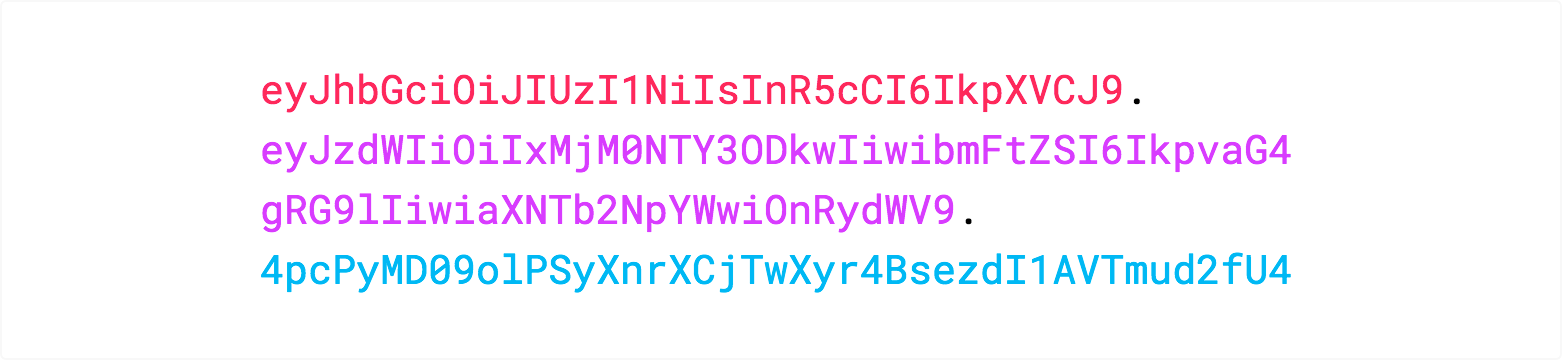
\includegraphics[width= \linewidth]{1.png}
    \captionof{figure}{Esempio token JWT}
    \vspace{2mm}
\end{minipage}

\end{center}

L'utente della nostra applicazione quindi una volta eseguito il login tramite il server di autenticazione riceverà come risposta un \textit{access\_token} rappresentato sotto forma di oggetto JWT tale per cui ogni volta che l'utente vuole effettuare l'accesso ad una risorsa protetta dovrà aggiungere all'header della richiesta il seguente:
\begin{center}

\fbox{
    Authorization: Bearer <JWT Token>
}
\end{center}

Il server, provider di servizi, comunicherà con il server di autenticazione in maniera tale da verificare l'autenticità del token ricevuto e quindi in funzione dell'autorizzazione concessa all'utente elargirà il servizio richiesto.

Un esempio di flusso di questo tipo è rappresentato infatti dalla seguente figura:

\begin{center}
\begin{minipage}{0.7\linewidth}
    \vspace{2mm}
    \centering
    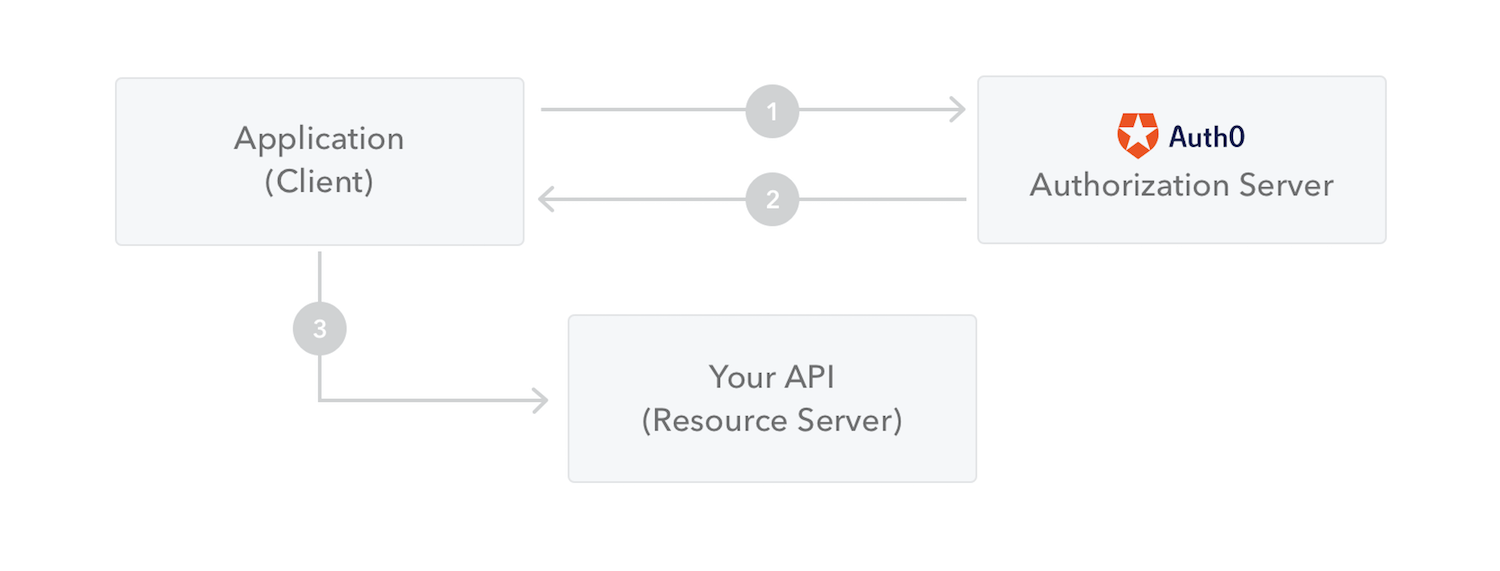
\includegraphics[width= \linewidth]{2.png}
    \captionof{figure}{Flusso di autorizzazione utente mediante richiesta token}
    \vspace{2mm}
\end{minipage}

\end{center}

Prima di procedere quindi ad eseguire un confronto tra JWT e SAML, è importante sottolineare che:

\begin{itemize}
    \item Il periodo di validità di un token JWT deve essere tale da garantire un compromesso tra usabilità e sicurezza. Di base, infatti, un token JWT scade dopo un periodo di 300 secondi (modificabile in funzione della necessità).
    \item Nonostante un token JWT sia signed, in assenza di uno strato di crittografia superiore, il suo contenuto è pubblicamente accessibile (non modificabile), per cui all'interno del payload JWT non dovrebbero essere inserite informazioni che devono rimanere segrete.
\end{itemize}

I vantaggi legati all'utilizzo di JWT piuttosto che la controparte SAML sono legati alle seguenti caratteristiche:

\begin{itemize}
    \item JSON è (molto) meno verboso di XML implicando così che la dimensione di un token codificato JWT risulta essere più efficiente in termini di spazio rispetto a SAML, garantendo così minor overhead quando questo viene trasferito tramite header HTTP.
    \item Da un punto di vista di sicurezza invece sia JWT che SAML presentano le medesime caratteristiche, tuttavia il processo di firma e crittografia di un token JWT risulta essere più semplice ed efficiente.
    \item Infine, proprio per la semplicità di interpretazione delle informazioni rappresentate sotto forma di documento JSON, ad oggi quasi ogni linguaggio di programmazione supporta un meccanismo di traduzione JSON-Object implicando così maggior semplicità nell'utilizzo dei token JWT.
\end{itemize}
\newpage
Di seguito è riportato un confronto delle dimensioni di un token JWT e l'equivalente SAML.

\begin{center}
\begin{minipage}{0.9\linewidth}
    \vspace{2mm}
    \centering
    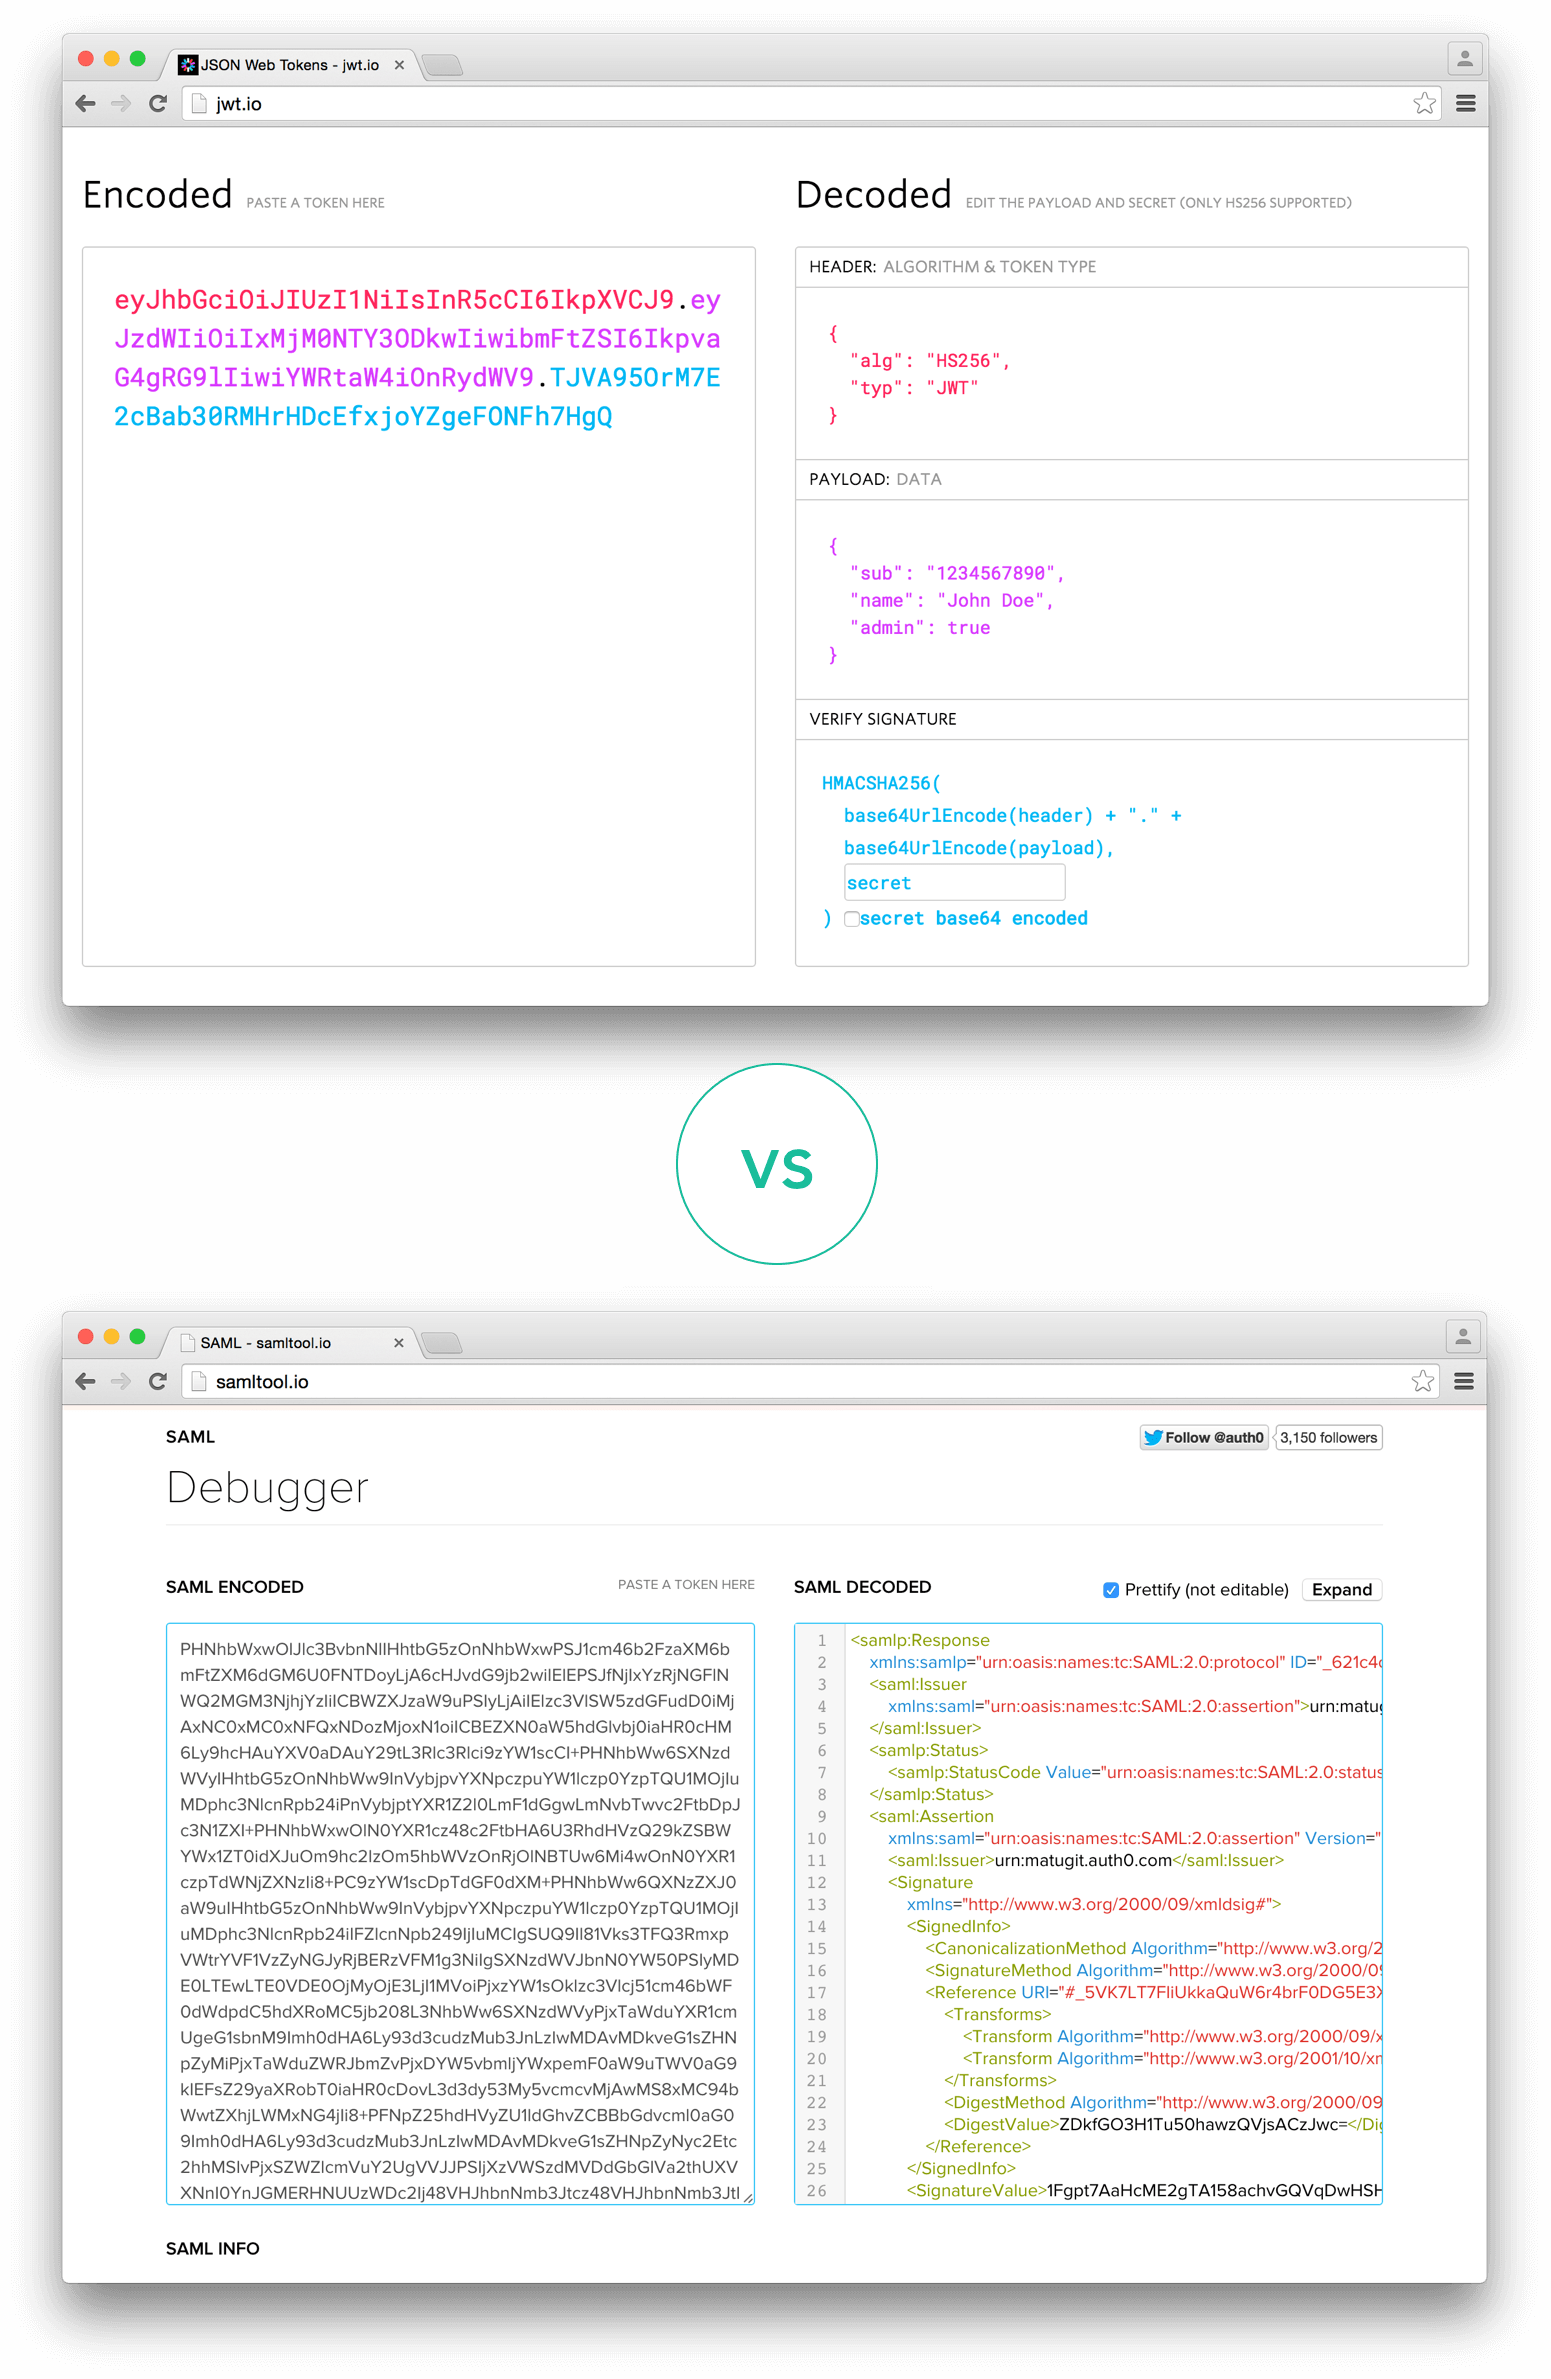
\includegraphics[width= \linewidth]{3.png}
    \captionof{figure}{JWT vs SAML}
    \vspace{2mm}
\end{minipage}

\end{center}

\section{Introduzione Docker}

\graphicspath{ {../progetto/images/docker/} }

Docker è una piattaforma open-source per lo sviluppo, il lancio e l'esecuzione delle applicazioni.

\begin{minipage}{\linewidth}
    \vspace{2mm}
    \centering
    
\includegraphics[width= \linewidth]{2.png}
    \captionof{figure}{Docker Logo}
    \vspace{2mm}
\end{minipage}

Docker permette di separare la specifica applicazione dall'infrastruttura su cui essa poggia così da ridurre significativamente il tempo necessario al rilascio del codice.
\bigbreak
Docker sfrutta un architettura client-server dove, il client interagisce (direttamente localmente o, nel caso in cui \textit{dockerd} fosse attivo su un host remoto, mediante REST API, Sockets o tramite interfaccia di rete) con un demone detto \textit{Docker Daemon} il cui compito è quello di buildare, eseguire e distribuire i container. 

\begin{minipage}{\linewidth}
    \vspace{2mm}
    \centering
    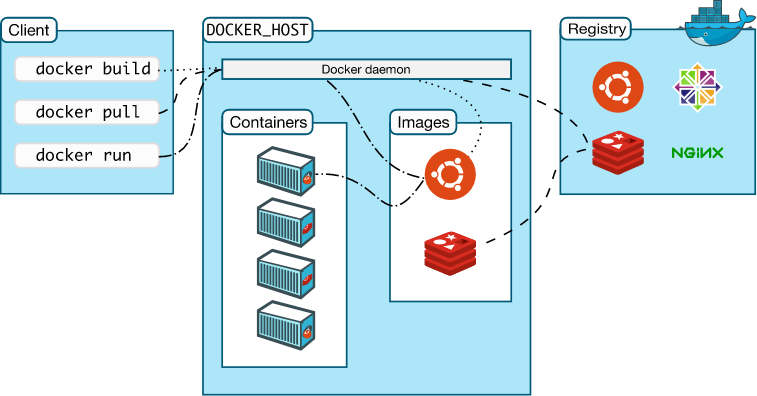
\includegraphics[width= \linewidth]{1.png}
    \captionof{figure}{Architettura Docker}
    \vspace{2mm}
\end{minipage}

Il vantaggio di utilizzare Docker è legato al fatto che le applicazioni sviluppate vengono appunto eseguite in ambienti chiamati 'Container' i quali garantiscono di lavorare con un sistema operativo virtualizzato senza dover gestire l'overhead legato alla virtualizzazione di un sistema operativo.
\bigbreak
Successivamente appunto verranno creati ed utilizzati una serie di container Docker con l'obiettivo di rendere più semplice il delivery di tale elaborato.




\chapter{Keycloak}
\thispagestyle{empty} 
\graphicspath{ {../progetto/images/keycloak/} }

\section{Introduzione a Keycloak}

Keycloak è una soluzione open-source per la gestione di autenticazione ed autorizzazione.
Esso presenta internamente un database relazionale utilizzato per gestire, conservare e interrogare le informazioni degli utenti.
\bigbreak

\begin{fancyquotes}
Add authentication to applications and secure services with minimum fuss.
No need to deal with storing users or authenticating users. It's all available out of the box.
\end{fancyquotes}

\bigbreak
Cioè che Keycloak permette di sviluppare un applicazione sicura senza dover affrontare la complessità di gestire internamente i differenti livelli di sicurezza associabili all'utente.
\bigbreak
Keycloak può essere riassunto in 3 differenti componenti:

\begin{enumerate}
    \item Realm: Un reame gestisce le informazioni legate alla sicurezza di un insieme di utenti, applicazioni e clients.
    \item Client: Un client rappresenta l'entità che può richiedere l'autenticazione di un utente in un determinato reame.
    \item Role: I ruoli identificano le differenti categorie di utenti, permettendo di applicare un controllo a grana fine sulle capabilities che possiede ognuna di esse nella nostra applicazione.
    Keycloak permette di gestire 3 differenti tipologie di ruoli che sono:
        \begin{itemize}
            \item Realm-Role level
            \item Client-Role level
            \item Composite-Role level che permette di comporre ruoli differenti fra loro e che verrà sfruttato successivamente per associare il ruolo a livello client al ruolo a livello reame.
        \end{itemize}
\end{enumerate}

\section{Docker e configurazione Keycloak}

Affinchè sia possibile interagire con keycloak bisogna configurare un server Keycloak. Per far ciò creiamo un container Docker.
\bigbreak
Avviamo quindi un ambiente Keycloak con username e password "admin" sfruttando il container "quay.io/keycloak/keycloak:15.0.2" su porta 5050

\begin{listing}[h!]
\begin{minted}[frame=single,
               framesep=3mm,
               bgcolor=white,
               numbersep=-10pt,
               ]{bash}
docker run
-p 5050:8080
-e KEYCLOAK_USER=admin
-e KEYCLOAK_PASSWORD=admin
quay.io/keycloak/keycloak:15.0.2
\end{minted} 
\end{listing}
\FloatBarrier

\bigbreak

a questo punto viene aperto in browser la pagina localhost:5050 dalla quale è possibile accedere a:


\begin{minipage}{\linewidth}
    \vspace{2mm}
    \centering
    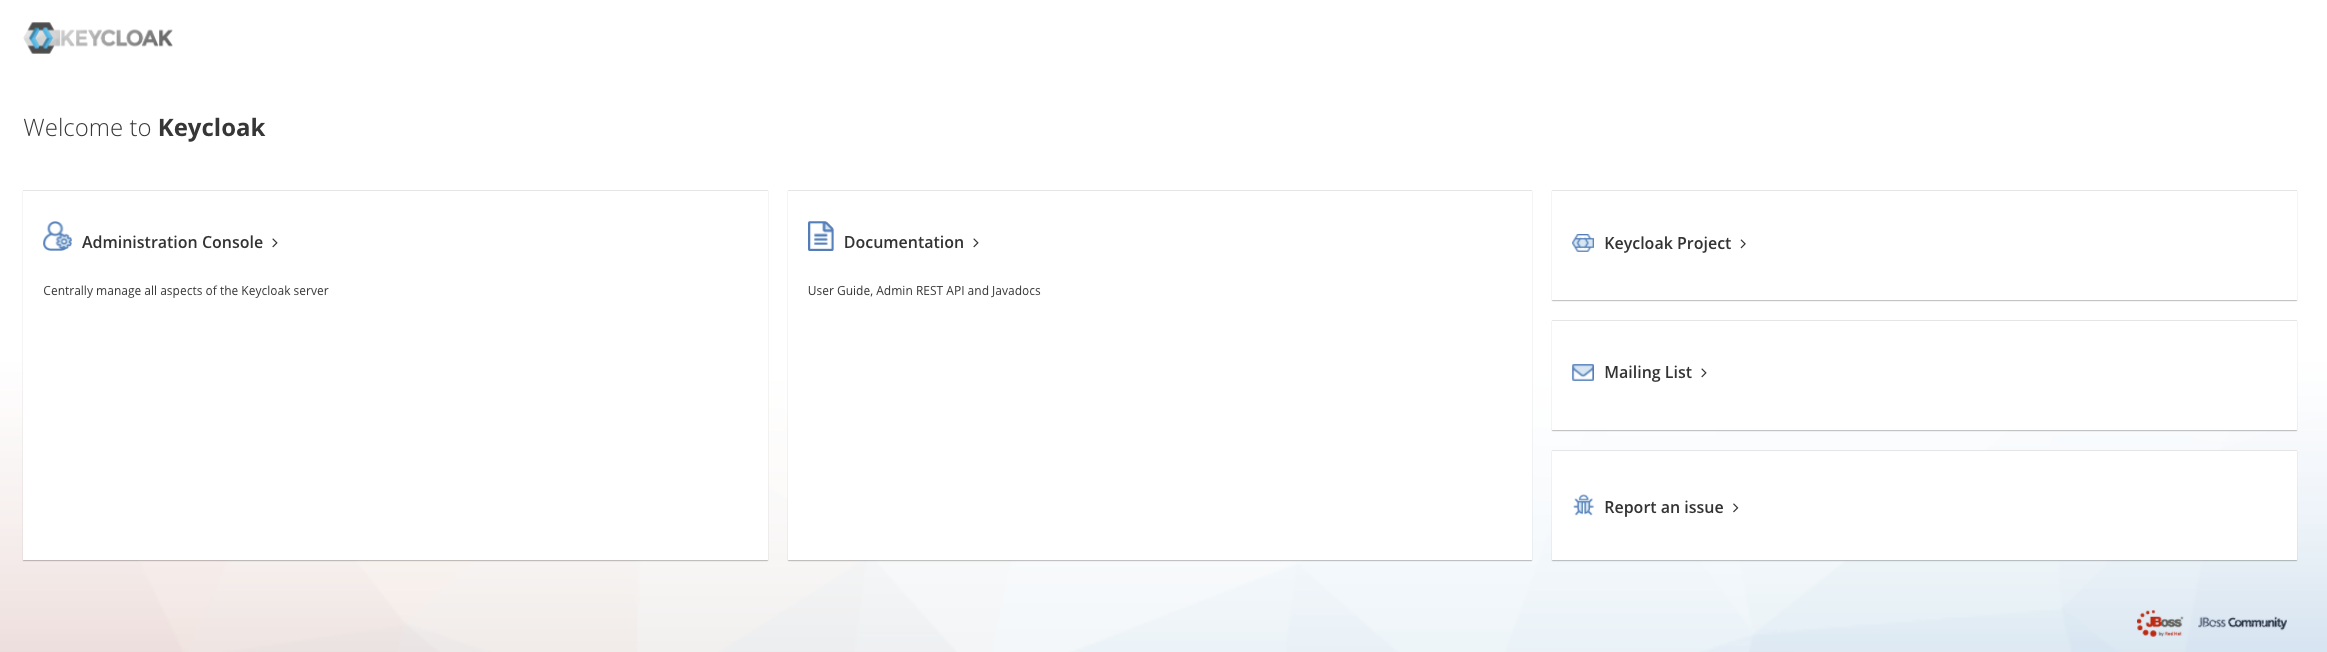
\includegraphics[width= \linewidth]{1.png}
    \captionof{figure}{Home page Keycloak}
    \vspace{2mm}
\end{minipage}

\begin{itemize}
	\item Administration Console
	\item Documentation
\end{itemize}


Oltre che a presentare una serie di hyperlinks per:


\begin{itemize}
	\item Accedere al Keycloak project (url che punta al sito ufficiale di keycloak)
	\item Accedere alla Mailing List
	\item Effettuare una segnalazione di malfunzionamento
\end{itemize}

Il prossimo passo quindi è quello di accedere al pannello di amministrazione tramite Administration Console.
\bigbreak
A questo punto si inseriscono le credenziali specificate su tale per cui:

\begin{itemize}
	\item username: admin
	\item password: admin
\end{itemize}


Una volta effettuato l'accesso sarà possibile accedere a differenti sezioni del progetto.


\begin{center}
\begin{minipage}{0.7\linewidth}
    \vspace{2mm}
    \centering
    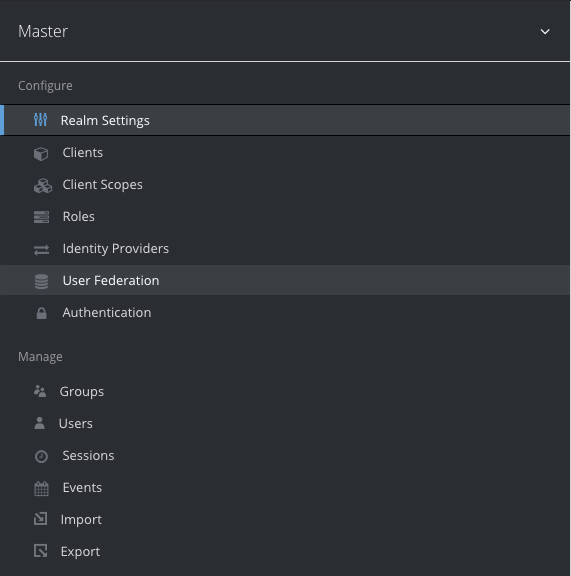
\includegraphics[width= \linewidth]{2.png}
    \captionof{figure}{Pannello di amministrazione del server Keycloak}
    \vspace{2mm}
\end{minipage}
\end{center}
\newpage
\section{Creazione di un Realm}

Un reame in Keycloak permette di creare degli ambienti isolati per la gestione di utenti e applicazioni. Keycloak stesso fa utilizzo di un reame "master" il quale è utilizzato per gestire le risorse keycloak.
\bigbreak
E' importante sottolineare che dal punto di vista pratico il realm "master" non dovrebbe essere utilizzato per applicazioni terze, le quali dovrebbero interagire con keycloak mediante un realm dedicato.
\bigbreak
Per creare un reame, bisogna fare hover sul dropdown che riporta il realm corrente e selezionare "add realm".

\begin{minipage}{\linewidth}
    \vspace{2mm}
    \centering
    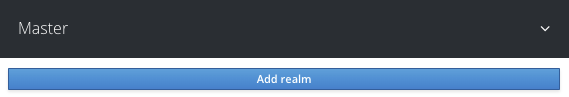
\includegraphics[width= \linewidth]{3.png}
    \captionof{figure}{Creazione nuovo Reame in Keycloak 1/2}
    \vspace{2mm}
\end{minipage}

Una volta selezionato "add realm", bisognerà specificare il nome del progetto a cui il realm è associato, nel nostro caso "SOASEC" e quindi procedere con la creazione del nuovo realm.

\begin{minipage}{\linewidth}
    \vspace{2mm}
    \centering
    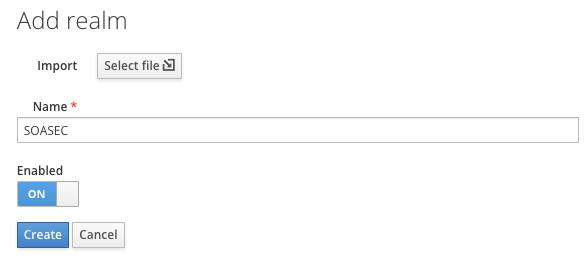
\includegraphics[width= \linewidth]{4.png}
    \captionof{figure}{Creazione nuovo Reame in Keycloak 2/2}
    \vspace{2mm}
\end{minipage}
\newpage
\section{Creazione di un nuovo user}

Appena creato il realm, il passo successivo sarà quello di creare un nuovo utente, con privilegi minori, il quale sarà in grado di accedere tramite keycloak alle applicazioni associate.
\bigbreak
Affinchè sia possibile creare un nuovo utente dobbiamo selezionare sotto la voce "Manage" il pulsante "Users" e quindi "Add User".

\begin{center}
\begin{minipage}{0.6\linewidth}
    \vspace{2mm}
    \centering
    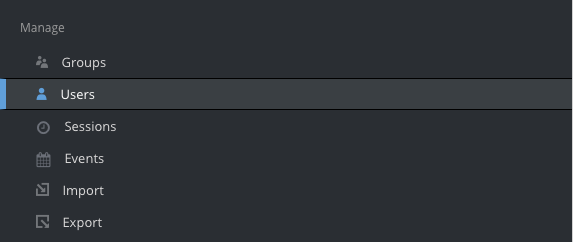
\includegraphics[width= \linewidth]{5.png}
    \captionof{figure}{Sezione Utenti}
    \vspace{2mm}
\end{minipage}
\end{center}

Vengono quindi inseriti i dati dell'utente come segue:

\begin{center}
\begin{minipage}{0.6\linewidth}
    \vspace{2mm}
    \centering
    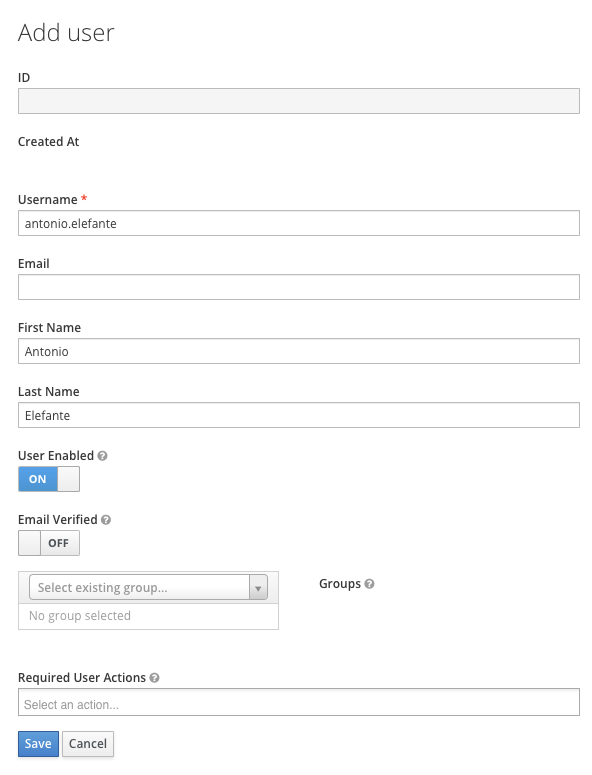
\includegraphics[width= \linewidth]{6.png}
    \captionof{figure}{Creazione di un nuovo utente}
    \vspace{2mm}
\end{minipage}
\end{center}

Si evidenzia che:
\begin{itemize}
\item L'unico campo non opzionale è rappresentato dal campo Username (associato ad un asterisco rosso)
\item L'utente può essere "abilitato" o "disabilitato", un utente disabilitato è un utente registrato il quale non può effettuare l'accesso alla piattaforma.
\item Si può specificare se la mail associata all'utente è una mail verificata (o alternativamente effettuare richiesta di verifica tramite la voce riportata all'ultimo punto)
\item E' possibile associare un utente ad un gruppo in maniera tale da permettere all'utente di ereditare determinate caratteristiche comuni al gruppo.
\item Infine, è possibile tramite la voce "Required User Actions" è possibile specificare delle operazioni che dovranno essere eseguite in maniera mandatoria da parte dell'utente, come ad esempio le seguenti:
	\begin{center}
    \begin{minipage}{0.7\linewidth}
        \vspace{2mm}
        \centering
        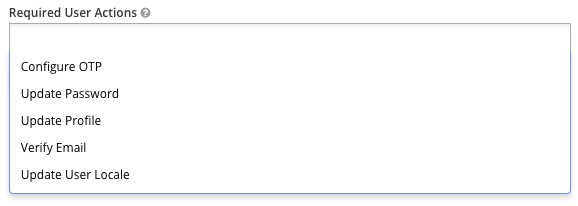
\includegraphics[width= \linewidth]{7.png}
        \captionof{figure}{Differenti azioni richiedibili all'utente}
        \vspace{2mm}
    \end{minipage}
    \end{center}
\end{itemize}
Una volta inseriti tutti i dati e confermate le opzioni associate, è possibile creare il nuovo utente tramite il pulsante "save" che ne attesta la creazione dell'utente ed il salvataggio delle varie informazioni associate allo stesso.
\bigbreak
Verrà quindi effettuato un redirect alla pagina di dettaglio dell'utente appena creato. Tale pagina di dettaglio ci permette di navigare le impostazioni associate all'utente tramite le seguenti voci:

\begin{center}
\begin{minipage}{0.6\linewidth}
    \vspace{2mm}
    \centering
    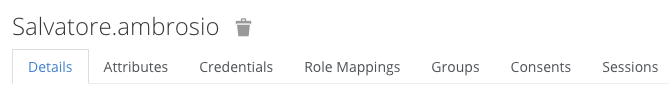
\includegraphics[width= \linewidth]{8.png}
    \captionof{figure}{Lista sezioni utente salvatore.ambrosio}
    \vspace{2mm}
\end{minipage}
\end{center}

Una volta giunti a tale fase, l'obiettivo attuale è quello di associare all'utente appena creato una nuova password, in maniera tale così da rendere possibile la fruizione dell'utente stesso presso le applicazioni descritte nei capitoli successivi.
\bigbreak
Per far ciò bisognerà navigare la dashboard utente alla voce "Credentials".

\begin{center}
\begin{minipage}{0.6\linewidth}
    \vspace{2mm}
    \centering
    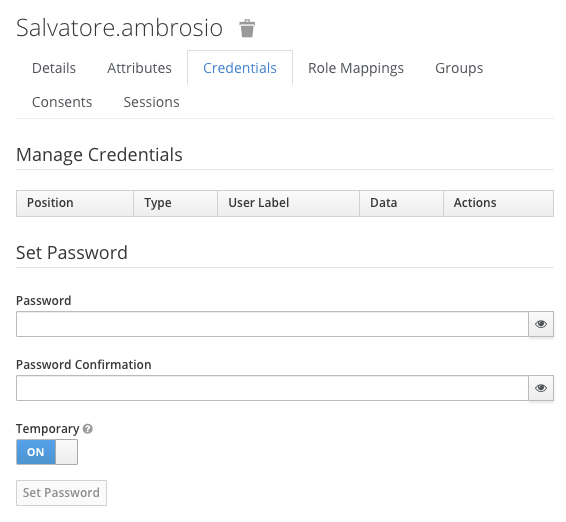
\includegraphics[width= \linewidth]{9.png}
    \captionof{figure}{Impostazione nuova password per l'utente salvatore.ambrosio 1/2}
    \vspace{2mm}
\end{minipage}
\end{center}

Tramite tale sezione sarà possibile inserire la password che l'utente potrà utilizzare per accedere all'ambiente Keycloak.
\bigbreak
E' importante sottolineare la possibilità di rendere tale password una password temporanea o definitiva. Nel caso in cui lo switch "Temporary" risultasse attivo, appena l'utente effettuerà il primo login, gli verrà richiesto di impostare una nuova password defintiva.
\bigbreak
Si procede dunque con l'associazione della password all'utente appena creato come in figura 2.10:

\begin{center}
\begin{minipage}{\linewidth}
    \vspace{2mm}
    \centering
    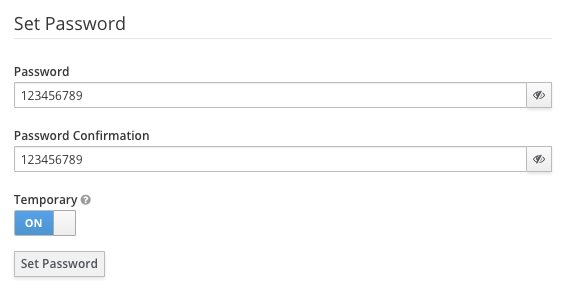
\includegraphics[width= \linewidth]{10.png}
    \captionof{figure}{Impostazione nuova password per l'utente salvatore.ambrosio 2/2}
    \vspace{2mm}
\end{minipage}
\end{center}

Keycloak utilizza l'algoritmo di hashing \textit{pbkdf2-sha256} che effettua un round di \textit{27500} iterazioni al fine di poter memorizzare la password in maniera sicura all'interno del database e proteggere tali password da un possibile leak.
\bigbreak
E' possibile osservare nella sezione di dettaglio account, che sotto la voce "Required Actions" è comparsa la spunta "Update Password". Questo è dovuto al fatto che la password precedentemente specificata era temporanea.
\bigbreak
Proviamo quindi ad effettuare l'accesso tramite le credenziali appena memorizzate tramite la Keycloak Account Console all'endpoint \textit{/auth/realms/SOASEC/account/}, e, come aspettato, il sistema ci presenta un form di aggiornamento della password. Tale operazione è necessaria per l'attivazione dell'utente.

\begin{center}
\begin{minipage}{0.6\linewidth}
    \vspace{2mm}
    \centering
    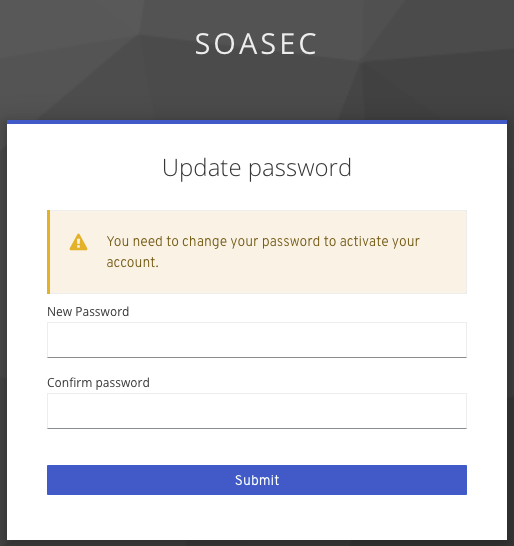
\includegraphics[width= \linewidth]{11.png}
    \captionof{figure}{Azione richiesta all'utente poichè password temporanea}
    \vspace{2mm}
\end{minipage}

\end{center}
Procediamo quindi con l'impostazione della nuova password (super) sicura

\begin{center}
\textit{Password123!}
\end{center}

Affinchè quindi sia possibile definire una determinata politica di accesso alla nostra applicazione e quindi consentire alla stessa di autenticare un utente risulterà necessario associavi un Client.

\section{Creazione di un Client}

I client sono le entità che possono richiedere a Keycloak di autenticare un utente. Molto spesso, i client sono associati ad applicazioni che vogliono usufruire di Keycloak per proteggere i servizi esposti sfruttando la tecnologia SSO (Single-Sign-On).
\bigbreak
Affinchè sia possibile creare un nuovo client bisogna selezionare la voce "Clients" sotto la sezione "Configure" e dunque dalla dashboard proposta cliccare sul pulsante "Create".

\begin{minipage}{\linewidth}
    \vspace{2mm}
    \centering
    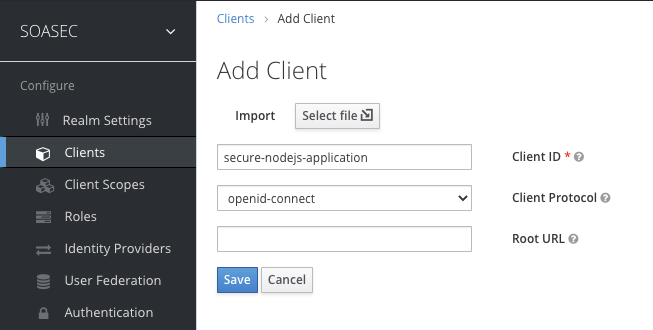
\includegraphics[width= \linewidth]{12.png}
    \captionof{figure}{Dashboard creazione client}
    \vspace{2mm}
\end{minipage}

Una volta specificato l'identificativo del client, possiamo concludere la creazione.
Si sottolinea che è una buona pratica associare all'identificativo del client una stringa rappresentativa dell'applicazione, in maniera tale da rendere più semplice la gestione nel caso in cui vi fossero svariati client nell'ecosistema SSO offerto da Keycloak.
\bigbreak
Creato il client, si imposta l'accesso come \textit{confidential} e si attivano i servizi \textit{Service Accounts Enabled} e \textit{Authorization Enabled}, fatto ciò saremo in grado di autenticare il client e quindi ottenere token dedicati per tale client.
\bigbreak
A questo punto si sarà in grado di recuperare sotto la voce \textit{Credentials} associata al client appena creato il \textit{Secret} associato allo stesso:
\begin{center}
\textit{e51bfd3e-6634-4319-bafa-e8022ee9f03b}
\end{center}

Keycloak rende quindi possibile definire dei ruoli per-client in maniera tale da poter associare a determinate API un determinato ruolo richiesto.
\bigbreak
Tipicamente infatti un applicazione presenta almeno due differenti ruoli, Utente ed Amministratore, per tale tipologia di applicazione dunque potrebbero essere esposte differenti tipologie di servizi sotto forma di API:
\begin{itemize}
\item Alcune API potrebbero essere pubblicamente accessibili
\item Alcune API potrebbero essere accessibili solo da Utenti
\item Alcune API potrebbero essere accessibili solo da Amministratori
\item Alcune API potrebbero essere accessibili sia da Utenti che Amministratori
\end{itemize}
Per tale motivazione dunque procediamo alla creazione di questi ruoli che utilizzeremo successivamente per autorizzare le richieste provenienti dall'esterno.

\section{Creazione di un ruolo associato ad un client in keycloak}

Affinchè sia possibile creare un nuovo ruolo in keycloak bisogna navigare la dashboard associata al client con identificativo \textit{secure-nodejs-application} alla sezione \textit{Roles} e dunque creare i ruoli:

\begin{itemize}
	\item user
	\item administrator
\end{itemize}

Corrediamo in entrambi i casi una breve descrizione del ruolo, in maniera tale da rendere più semplice la manutenzione in presenza di più ruoli associati ad un singolo client.

\begin{minipage}{\linewidth}
    \vspace{2mm}
    \centering
    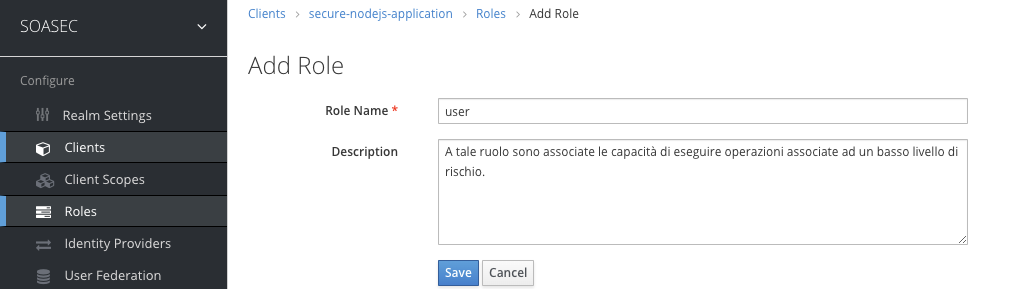
\includegraphics[width= \linewidth]{13.png}
    \captionof{figure}{Creazione client-role}
    \vspace{2mm}
\end{minipage}

Viene quindi creato anche il ruolo \textit{app-user}.
\bigbreak
In figura è quindi riportato un riepilogo dei ruoli attualmente presenti ed associati al client \textit{secure-nodejs-application}.

\begin{minipage}{\linewidth}
    \vspace{2mm}
    \centering
    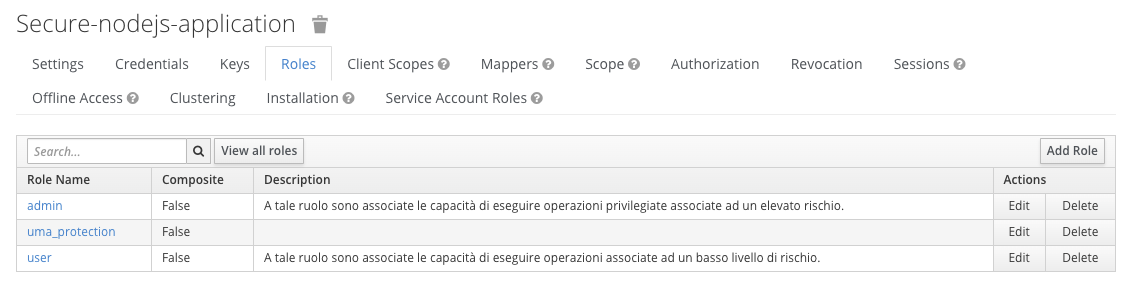
\includegraphics[width= \linewidth]{14.png}
    \captionof{figure}{Lista ruoli per client d'esempio}
    \vspace{2mm}
\end{minipage}

In maniera analoga per il Realm, è possibile creare dei ruoli app-specific, i quali saranno associati ai ruoli appena creati.
\bigbreak
Questo perchè spesso le applicazioni garantiscono accesso e autorizzazione a specifici ruoli, piuttosto che ad utenti in quanto un controllo di questo tipo potrebbe essere un controllo a grana troppo fine, diventando così difficile da manutenere all'aumentare del numero degli utenti della nostra applicazione.
\bigbreak
Per far ciò dunque selezioniamo dalla sezione \textit{Configure} la voce \textit{Realms} ed a questo punto creiamo i ruoli app-specific che saranno:

\begin{itemize}
	\item app-user
	\item app-administrator
\end{itemize}

Una volta aggiunti tali ruoli, li rendiamo \textit{Composite Role} ed associamo ad entrambi il rispettivo \textit{Client role}.

\begin{minipage}{\linewidth}
    \vspace{2mm}
    \centering
    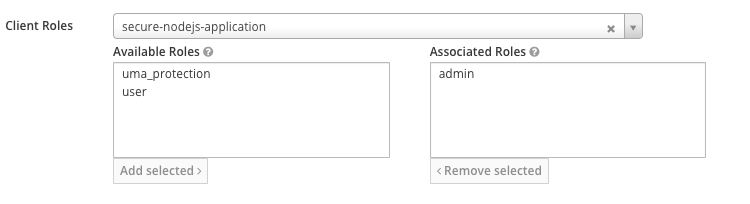
\includegraphics[width= \linewidth]{15.png}
    \captionof{figure}{Role composition, associazione realm role app-administrator al client role admin}
    \vspace{2mm}
\end{minipage} 

\section{Creazione utenti ed associazione ruoli}

Come detto precedentemente, gli utenti sono le entità che possono eseguire accesso al sistema. Ad ogni utente possono essere associati differenti attributi, come username, email, nome, cognome etc e possono essere associati a gruppi o essere assegnabili a specifici ruoli.
\bigbreak
Ciò che faremo quindi sarà quello di associare agli utenti precedentemente creati

\begin{itemize}
	\item antonio.elefante
	\item salvatore.ambrosio
\end{itemize}

dei ruoli, in maniera tale così da poter sfruttare tali ruoli per interagire successivamente con il sistema.
\bigbreak
Per far ciò basterà selezionare l'utente a cui vogliamo associare il ruolo, e conseguentemente sotto la sezione \textit{Role Mappings} specificare la categoria desiderata.
\bigbreak
Ad esempio, procediamo con l'assegnazione del ruolo \textit{app-administrator} all'utente caratterizzato dall'username \textit{antonio.elefante}.

\begin{minipage}{\linewidth}
    \vspace{2mm}
    \centering
    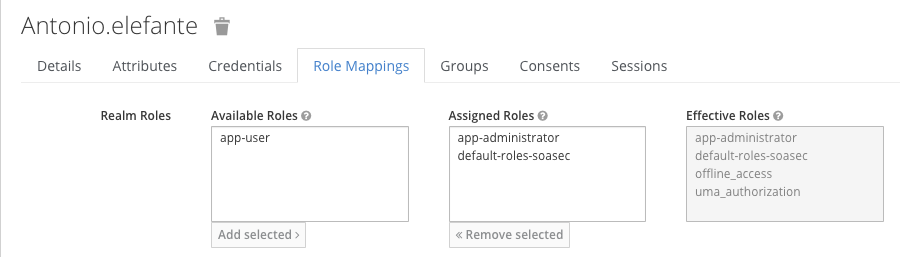
\includegraphics[width= \linewidth]{16.png}
    \captionof{figure}{Ruoli associati all'utente antonio.elefante}
    \vspace{2mm}
\end{minipage} 

In maniera analoga, associamo all'utente \textit{salvatore.ambrosio} il ruolo \textit{app-user}

\subsection{Come ottenere un token una volta definito un realm ed i relativi utenti}

Affinchè sia possibile recuperare il token di autorizzazione, bisogna preventivamente determinare qual è l'endpoint utile per poter richiedere a Keycloak lo stesso.
\bigbreak
Per far ciò bisognerà selezionare \textit{Realm settings} dal pannello laterale e quindi cliccare sul collegamento \textit{OpenID Endpoint Configuration}.
\bigbreak
Tale link punta ad un endpoint il quale fornisce in output una stringa in formato JSON.
\bigbreak
Di tale stringa JSON ci interessa la chiave \textit{token\_endpoint} da cui:
\begin{listing}[h!]
\begin{minted}[frame=single,
               framesep=3mm,
               bgcolor=white,
               numbersep=-10pt,
               ]{json}
{
  "...":"...",
  "token_endpoint":"http://base_url:port/auth/realms
  /REALM/protocol/openid-connect/token",
  "...":"...",
}
\end{minted}
\end{listing}
\FloatBarrier

\bigbreak


E' possibile quindi ottenere l'access token semplicemente effettuando una richiesta http POST fornendo i seguenti valori di input:



\begin{table}[h]
\centering
\begin{tabular}{|r|l|}
\hline
\textbf{grant\_type} & password            \\ \hline
\textbf{client\_id}    & secure-nodejs-application   \\ \hline
\textbf{client\_secret}    & e51bfd3e-6634-4319-bafa-e8022ee9f03b  \\ \hline
\textbf{username}   & antonio.elefante \\ \hline
\textbf{password}   & 123456789 \\ \hline
\end{tabular}
\captionof{table}{Coppie Key-Value necessari per l'ottenimento del token JWT}
\end{table}
\FloatBarrier

\bigbreak

Tale richiesta fornirà in output una stringa in formato JSON contenente in particolare i seguenti:

\begin{itemize}
	\item \textit{access\_token}: Il token in formato JWT
	\item \textit{expires\_in}: Il tempo di validità del token appena ricevuto, una volta esaurito tale tempo le richieste effettuate risponderanno con \textit{http code 401-unauthorized}
\end{itemize}

Tale token può essere autonomamente decodificato tramite \href{https://jwt.io/}{\underline{jwt.io}} e riporta alcuni riferimenti all'utente processato, fra cui il ruolo ad esso associato.
\bigbreak
E' importante sottolineare che Keycloak permette di modificare l'algoritmo di generazione dei token come ad esempio per aumentare o diminuire la durata di validità del token stesso.
\bigbreak
Una volta completati tali passaggi, eseguiamo un \textit{docker commit} delle modifiche effettuate al server così da poter congelare lo stato attuale del server keycloak e quindi successivamente poter utilizzare il seguente comando per poter riprendere dallo stato attuale:

\begin{listing}[h!]
\begin{minted}[
frame=single,
framesep=3mm,
bgcolor=white,
numbersep=-10pt,               
]{bash}
docker run 
-p 5050:8080
-e KEYCLOAK_USER=admin
-e KEYCLOAK_PASSWORD=admin
soasec/keycloak
\end{minted} 
\end{listing}
\FloatBarrier

\bigbreak

\begin{minipage}{\linewidth}
    \vspace{2mm}
    \centering
    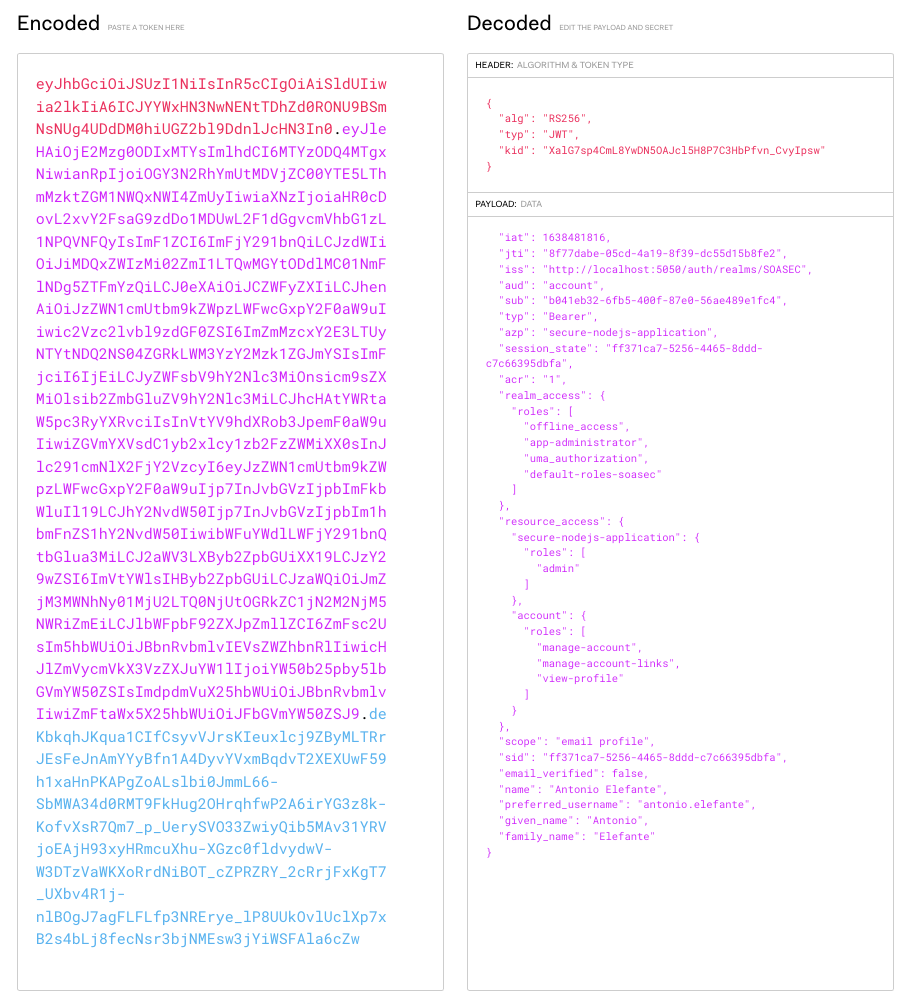
\includegraphics[width= \linewidth]{17.png}
    \captionof{figure}{Esempio token JWT ottenuto dall'autenticazione tramite Keycloak}
    \vspace{2mm}
\end{minipage} 

\chapter{Progetto Back-End}
\thispagestyle{empty} 
\graphicspath{ {../progetto/images/nodejs/} }
\section{NodeJS}
\subsection{Introduzione a NodeJS}

NodeJS è un runtime environment JavaScript open-source e cross-platform.

\begin{center}
\begin{minipage}{0.75\linewidth}
    \vspace{2mm}
    \centering
    
\includegraphics[width= \linewidth]{1.png}
    \captionof{figure}{NodeJS logo}
    \vspace{2mm}
\end{minipage}
\end{center}

Node.js sfrutta a pieno il motore JavaScript V8 sviluppato per rendere più efficiente l'interpretazione del codice JavaScript nel browser Google Chrome.
\bigbreak
Un'applicazione NodeJS viene eseguita interamente in un singolo processo, permettendo, tramite un insieme di primitive asincrone di I/O di sviluppare codice non bloccante in grado di rispondere a numerose richieste senza la necessità di creare un nuovo thread per ogni richiesta sopraggiunta.
\bigbreak
Ciò permette a NodeJS di poter rispondere a migliaia di richieste concorrenti senza la necessità di dover gestire la concorrenza fra differenti thread che, talvolta, può portare all'introduzione di bugs che potrebbero essere difficili da risolvere.

\subsection{Applicazione pratica}

Anche in questo caso viene fatto utilizzo di docker al fine di rendere il lavoro effettuato non solo semplice da manutenere, data proprio la caratteristica di docker nel rendere deterministico il funzionamento di un dato sistema, ma anche di rendere semplice il trasferimento dell'intero progetto.
\bigbreak
Creiamo quindi un nuovo progetto nodejs mediante il comando \textit{npm init} il quale ci fa definire una serie di informazioni associate al progetto stesso.


\begin{listing}[h!]
\begin{minted}[frame=single,
               framesep=3mm,
               bgcolor=white,
               numbersep=-10pt,
               ]{json}
{
  "name": "progetto-soasec",
  "version": "1.0.0",
  "description": "Progetto SOASEC: 
  NodeJS (Back-End), 
  MongoDB (DB NoSQL), 
  Keycloak (Authentication+Authorization), 
  Flutter (Front-End)",
  "main": "index.js",
  "scripts": {
    "start": "nodemon index.js"
  },
  "author": "Antonio Elefante, Salvatore Ambrosio",
  "license": "ISC"
}
\end{minted}
\end{listing}
\FloatBarrier
Creiamo un file index.js che rappresenterà la nostra applicazione NodeJS mediante il comando \textit{touch index.js} ed il DockerFile, \textit{touch DockerFile}. 

\begin{listing}[h!]
\begin{minted}[frame=single,
               framesep=3mm,
               bgcolor=white,
               numbersep=-10pt,
               ]{Dockerfile}
FROM node:17

# Create app directory
WORKDIR /usr/src/app

# Install app dependencies
# A wildcard is used to ensure both 
# package.json and package-lock.json are copied
# where available (npm@5+)
COPY package*.json ./

RUN npm install

# Bundle app source
COPY . .

EXPOSE 8080
CMD [ "node", "index.js" ]
\end{minted}
\end{listing}
\FloatBarrier

Affinchè sia possibile esporre delle API tramite framework back-end NodeJS bisognerà far utilizzo del package \textit{express} il quale fornisce le metodologie per la creazione di un listener, l'interpretazione della richiesta e la generazione di risposta su protocollo http/https.
\bigbreak
Pertanto tramite il seguente comando installiamo le dipendenze necessarie per l'utilizzo di express:

\begin{listing}[h!]
\begin{minted}[frame=single,
               framesep=3mm,
               bgcolor=white,
               numbersep=-10pt,
               ]{bash}
npm install express
\end{minted}
\end{listing}
\FloatBarrier

A questo punto saremo in grado di creare ed utilizzare un applicazione express mediante il seguente codice, il cui scopo è semplicemente quello di creare un server in ascolto su porta 8080 in grado di rispondere alla sola richiesta \textit{http://base\_url:port/} con un semplice messaggio di stato.

\begin{listing}[h!]
\begin{minted}[frame=single,
               framesep=3mm,
               bgcolor=white,
               numbersep=-10pt,
               ]{js}
var express = require('express');
var app = express();

app.get('/', function(req, res){
   res.send("Il server è attivo e funzionante!");
});

app.listen(8080);
\end{minted}
\end{listing}
\FloatBarrier

Una volta verificata la raggiungibilità del server si andrà ad aggiungere funzionalità al fine di esporre la seguente lista di servizi:

\begin{itemize}

    \item Visualizzazione lista candidati (public/anonymous)
    \item Votazione candidato (app-user)
    \item Aggiunta nuovo candidato (app-admin)

\end{itemize}

Per far ciò dunque strutturiamo il progetto mediante la seguente struttura ad albero:

\begin{center}

\begin{forest}
  [Base Folder
    [index.js]
    [Routes
        [anonymous-routes.js] [user-routes.js] [admin-routes.js]
    ]
  ]
\end{forest}

\end{center}

Nello specifico, i files \textit{*-routes.js} presenteranno una struttura simile, utile per poter esporre determinati servizi.
\bigbreak
Tale caratteristica infatti è legata alla modalità in cui i \textit{moduli} sono gestiti da NodeJS. Ogni modulo infatti richiederà solo ed esclusivamente i package da esso richiesti per poter funzionare, e quindi esporrà all'esterno solo i metodi necessari al corretto funzionamento della funzionalità che si vuole esporre.
\newpage
Un esempio di file *-routes.js è il seguente:
\begin{listing}[h!]
\begin{minted}[frame=single,
               framesep=3mm,
               bgcolor=white,
               numbersep=-10pt,
               ]{js}
var express = require('express');
var router = express.Router();

router.get('/route', function(req, res){
    res.send("Ottimo, hai raggiunto la rotta 
        http://base_url/nome_modulo/route");
});

module.exports = router;
\end{minted}
\end{listing}
\FloatBarrier

Una volta definite le rotte esposte dai singoli files, possiamo integrarle facilmente nella nostra applicazione semplicemente segnalando all'applicazione di usufruire delle determinate rotte.
\bigbreak
Per far ciò bisogna quindi:

\begin{itemize}
    \item[1.] Importare il file tramite require(file)
    \item[2.] Utilizzare le funzionalità esposte dal modulo importato.
\end{itemize}


\begin{listing}[h!]
\begin{minted}[frame=single,
               framesep=3mm,
               bgcolor=white,
               numbersep=-10pt,
               ]{js}
var anonymous_routes = require('./Routes/
    anonymous-routes.js');
var user_routes = require('./Routes/
    user-routes.js');
var admin_routes = require('./Routes/
    admin-routes.js');

app.use('/anonymous', anonymous_routes);
app.use('/user', user_routes);
app.use('/admin', admin_routes);

\end{minted}
\end{listing}
\FloatBarrier

Il problema però è legato al fatto che la semplice strutturazione del progetto non garantisce alcuna funzionalità, ne alcun livello di sicurezza.
\bigbreak
Nello specifico, per poter aggiungere funzionalità al progetto, collegheremo alla nostra applicazione NodeJS un database di tipo NoSQL il quale verrà utilizzato per memorizzare sotto forma di documenti JSON le informazioni relative alla votazione.
\bigbreak
Viceversa, per quanto riguarda la sicurezza, proteggeremo le API con i relativi ruoli mediante Keycloak.

\section{Proteggere le APIs tramite Keycloak}

Per poter proteggere le API precedentemente esposte pubblicamente tramite server NodeJS bisogna far utilizzo dei seguenti:

\begin{itemize}
    \item keycloak-connect
    \item express-session
\end{itemize}

Dove, nello specifico, keycloak-connect deve essere configurato in maniera tale da rendere raggiungibile lo specifico server keycloak. Una volta configurato possiamo sfruttare il middleware \textit{keycloak.protect(...)} per aggiungere il layer di sicurezza alle API esposte.

\begin{listing}[h!]
\begin{minted}[frame=single,
               framesep=3mm,
               bgcolor=white,
               numbersep=-10pt,
               ]{bash}
npm install keycloak-connect
npm install express-session
\end{minted}
\end{listing}
\FloatBarrier

Viene quindi creata una nuova cartella all'interno del progetto al fine di rendere più semplice la strutturazione del codice.

\begin{center}

\begin{forest}
  [Base Folder
    [index.js]
    [Routes
        [anonymous-routes.js] [user-routes.js] [admin-routes.js]
    ]
    [Keycloak
        [keycloak-config.js]
    ]
  ]
\end{forest}

\end{center}

In particolare si specifica che per finalità progettuali, le informazioni come le chiavi private vengono inserite in maniera cable-coded all'interno del progetto, tuttavia però in ambiente di produzione, sarebbe più opportuno far utilizzo del pacchetto \textit{dotenv} il quale ci permette di memorizzare le chiavi private in un file, appunto chiamato \textit{.env} il quale verrà blacklistato all'interno del file \textit{.gitignore}. Tutto questo per rendere quanto meno possibile pubbliche informazioni che dovrebbero rimanere private.
\bigbreak
Procediamo quindi con l'analisi del file \textit{keycloak-config.js}.
\bigbreak
Anzitutto, come anticipato sarà necessario importare i moduli keycloak-connect e express-session:

\begin{listing}[h!]
\begin{minted}[frame=single,
               framesep=3mm,
               bgcolor=white,
               numbersep=-10pt,
               ]{js}
var session = require('express-session');
var Keycloak = require('keycloak-connect');
\end{minted} 
\end{listing}
\FloatBarrier

Una volta importati, procediamo quindi con la specificazione dei parametri di configurazione di keycloak:

\begin{listing}[h!]
\begin{minted}[frame=single,
               framesep=3mm,
               bgcolor=white,
               numbersep=-10pt,
               ]{js}
var keycloakConfig = {
    clientId: 'secure-nodejs-application',
    bearerOnly: true,
    serverUrl: 'http://localhost:5050/auth',
    realm: 'SOASEC',
    credentials: {
        secret: 'e51bfd3e-6634-4319-bafa-e8022ee9f03b'
    }
};

\end{minted}
\end{listing}
\FloatBarrier

Viene quindi definita una funzione per ottenere accesso all'oggetto Keycloak:

\begin{listing}[h!]
\begin{minted}[frame=single,
               framesep=3mm,
               bgcolor=white,
               numbersep=-10pt,
               ]{js}
let _keycloak;
function getKeycloak() {
    if (_keycloak) {
        console.log("Keycloak già inizializzato");
        return _keycloak;
    } 
    else {
        console.log("Inizializzazione 
            connessione al server Keycloak...");
        var memoryStore = new session.MemoryStore();
        _keycloak = new Keycloak(
        { 
            store: memoryStore
        }, keycloakConfig);
        return _keycloak;
    }
}

\end{minted}
\end{listing}
\FloatBarrier

Fatto ciò, non ci resta altro che esporre l'accesso alla funzione \textit{getKeycloak()} all'esterno:

\begin{listing}[h!]
\begin{minted}[frame=single,
               framesep=3mm,
               bgcolor=white,
               numbersep=-10pt,
               ]{js}

module.exports = {
    getKeycloak
}

\end{minted}
\end{listing}
\FloatBarrier

Ora modifichiamo il file index.js al fine di integrare quanto appena fatto con le seguenti modifiche:

\begin{listing}[h!]
\begin{minted}[frame=single,
               framesep=3mm,
               bgcolor=white,
               numbersep=-10pt,
               ]{js}

const keycloak = require('./Keycloak/
    keycloak-config.js').getKeycloak();
app.use(keycloak.middleware());
\end{minted}
\end{listing}
\FloatBarrier

E quindi implementiamo infine una politica di accesso alle API basata su ruoli mediante l'impiego del middleware come segue:

\begin{listing}[h!]
\begin{minted}[frame=single,
               framesep=3mm,
               bgcolor=white,
               numbersep=-10pt,
               ]{js}

app.use('/anonymous', anonymous_routes);
app.use('/user', keycloak.protect("user"),user_routes);
app.use('/admin', keycloak.protect("admin"),
    admin_routes);

\end{minted}
\end{listing}
\FloatBarrier
\graphicspath{ {../progetto/images/mongodb/} }
\section{Connessione al database NoSQL MongoDB}
\subsection{Introduzione MongoDB}

\begin{center}
\begin{minipage}{0.75\linewidth}
    \vspace{2mm}
    \centering
    
\includegraphics[width= \linewidth]{1.png}
    \captionof{figure}{MongoDB logo}
    \vspace{2mm}
\end{minipage}
\end{center}

MongoDB è un database NoSQL orientato ai documenti, che nasce nel 2007 in California come servizio da utilizzare nell'ambito di un progetto più ampio, ma che presto è diventato un prodotto indipendente ed open-source. MongoDB memorizza le informazioni sotto forma di documenti i quali sono a loro volta rappresentati mediante formato JSON.
\bigbreak
Le caratteristiche chiave di MongoDB sono:

\begin{itemize}
\item Alta replicabilità
\item Altamente scalabile: MongoDB infatti permette di distribuire i documenti su più nodi in modo tale così da supportare grandi quantità di dati senza impattare negativamente sulle performance globali del sistema.
\end{itemize}

MongoDB si adatta a molti contesti, in generale quando si manipolano grandi quantità di dati eterogenei e senza uno schema ben definito. 
\bigbreak
Non è invece opportuno quando si devono gestire molte relazioni tra oggetti, e si vuole garantire l’integrità referenziale tra essi.

\subsection{Applicazione pratica}

Affinchè sia possibile connettere il server NodeJS ad una base dati MongoDB vi sono due differenti possibilità:

\begin{itemize}
    \item[1.] Creare una istanza Atlas gratuita presso MongoDB
    \item[2.] Creare ed eseguire un istanza locale
\end{itemize}

Ovviamente, per le finalità che si vogliono raggiungere risulta più comodo avviare una istanza locale di MongoDB mediante container Docker.
\bigbreak
Per far ciò scarichiamo ed eseguiamo una nuova istanza MongoDB mediante i seguenti comandi:

\begin{listing}[h!]
\begin{minted}[frame=single,
               framesep=3mm,
               bgcolor=white,
               numbersep=-10pt,
               ]{bash}
docker pull mongo
\end{minted}
\end{listing}
\FloatBarrier

E successivamente avviamo l'istanza mongo tramite il seguente:
\begin{listing}[h!]
\begin{minted}[frame=single,
               framesep=3mm,
               bgcolor=white,
               numbersep=-10pt,
               ]{bash}
docker run 
-p 6060:27017 
-d mongo
\end{minted}
\end{listing}
\FloatBarrier


A questo punto, sempre da terminale all'interno della cartella in cui è sito il progetto è possibile eseguire il seguente comando che associerà al progetto la dipendenza da MongoDB:

\begin{listing}[h!]
\begin{minted}[frame=single,
               framesep=3mm,
               bgcolor=white,
               numbersep=-10pt,
               ]{bash}
npm install mongoose
\end{minted}
\end{listing}
\FloatBarrier

Una volta fatto ciò si potrà importare dove necessario il \textit{package mongoose} il quale potrà essere sfruttato come \textit{driver} per le comunicazioni con il database:

\begin{listing}[h!]
\begin{minted}[frame=single,
               framesep=3mm,
               bgcolor=white,
               numbersep=-10pt,
               ]{js}

var mongoose = require('mongoose');
var mongoDB = 'mongodb://base_url/database';
mongoose.connect(mongoDB, 
    {
        useNewUrlParser: true,
        useUnifiedTopology: true
    }
);

\end{minted}
\end{listing}
\FloatBarrier

Non ci resta quindi che definire e strutturare lo schema del database, così da poter interagire ed applicare maggiori controlli ai dati che dovranno essere memorizzati.
\bigbreak
Le informazioni che verranno quindi memorizzate all'interno del database sfrutteranno il seguente schema:

\begin{table}[h]
\centering
\begin{tabular}{|c|}
\hline
\textbf{Candidato} \\ \hline
nome   \\ \hline
cognome  \\ \hline
votanti  \\ \hline
\end{tabular}
\captionof{table}{Candidato Schema}
\end{table}
\FloatBarrier

E' importante sottolineare che in un progetto reale, un database costituito da questa singola tabella risulterebbe essere inutile, tuttavia una base dati di questo tipo risulta sufficiente a garantire un livello di astrazione tale da dimostrare di aver compreso le modalità di protezione delle API CRUD.
\bigbreak
Per tale motivazione quindi viene creata la cartella \textit{Model} e quindi definiti all'interno di tale cartella il file necessario alla gestione dello schema appena presentato:


\begin{center}
\resizebox{\textwidth}{!}{%
\begin{forest}
  [Base Folder
    [index.js]
    [Routes
        [anonymous-routes.js] [user-routes.js] [admin-routes.js]
    ]
    [Keycloak
        [keycloak-config.js]
    ]
    [Model
        [candidato-model.js]
    ]
  ]
\end{forest}}

\end{center}

Di cui, il file candidato-model.js conterrà il seguente snippet:

\begin{listing}[h!]
\begin{minted}[frame=single,
               framesep=3mm,
               bgcolor=white,
               numbersep=-10pt,
               ]{js}

const mongoose = require('mongoose')

const Candidato = new mongoose.Schema({
    nome: {
        type: 'String',
        required: true
    },
    cognome: {
        type: 'String',
        required: true
    },
    votanti: [{ 
        type: 'String'
    }]
})

module.exports = mongoose.model("Candidati", Candidato)
\end{minted}
\end{listing}
\FloatBarrier

Una volta fatto ciò, basterà utilizzare tale schema all'interno dei metodi precedentemente definiti al fine di garantire una corretta funzionalità degli stessi.
\bigbreak
Per semplicità viene riportato solo un esempio di API (\textbf{C}RUD Creazione nuovo candidato), rimandando al lettore la possibilità di osservare il progetto nella sua interezza.

\begin{listing}[h!]
\begin{minted}[frame=single,
               framesep=3mm,
               bgcolor=white,
               numbersep=-10pt,
               ]{js}
var express = require('express');
var router = express.Router();
var Candidato = require('../Model/candidato-model.js')

router.get('/creazione-nuovo-candidato', 
    function(req, res){
        try {
            const nuovoCandidato = new Candidato({
                'nome': req.body.nome,
                'cognome': req.body.cognome,
                'votanti': []
            });
            await nuovoCandidato.save();
            res.send(
                {
                    "error":"false",
                    "message":"candidato
                     creato correttamente"
                }
            )
        } catch (err) {
          res.status(500).send(err);
        }
    }
);

module.exports = router;
\end{minted}
\end{listing}
\FloatBarrier

Una volta definita l'implementazione delle API, è possibile trasformare tale progetto in un container docker al fine di rendere completo e finale il progetto Back-End.
\bigbreak
Per far ciò definiamo il file \textit{.dockerignore} al fine di ignorare la copia locale dei package installati tramite npm (\textit{node package manager}) ed infine viene creata la build del container docker:

\begin{listing}[h!]
\begin{minted}[frame=single,
               framesep=3mm,
               bgcolor=white,
               numbersep=-10pt,
               ]{bash}
docker build . 
-t soasec/nodejs-application
\end{minted}
\end{listing}
\FloatBarrier

A questo punto possiamo eseguire l'applicazione tramite docker mediante il seguente comando:

\begin{listing}[h!]
\begin{minted}[frame=single,
               framesep=3mm,
               bgcolor=white,
               numbersep=-10pt,
               ]{bash}
docker run 
-p 49160:8080 
-d soasec/nodejs-application
\end{minted}
\end{listing}
\FloatBarrier

\chapter{Progetto Front-End}
\thispagestyle{empty} 
\section{Flutter}

\graphicspath{ {../progetto/images/flutter/} }

\subsection{Introduzione}

\begin{minipage}{\linewidth}
    \vspace{2mm}
    \centering
    
\includegraphics[width= \linewidth]{icon.png}
    \captionof{figure}{Flutter logo}
    \vspace{2mm}
\end{minipage}

Flutter è un framework open-source creato da Google per lo sviluppo front-end di interfacce grafiche native per iOS e Android, oltre ad essere il metodo principale per la creazione di applicazioni per Google Fuchsia.
\bigbreak
Con la versione 1.9, Google introduce il supporto per le applicazioni web e per siti statici scritti in linguaggio Dart. 
\bigbreak
Tra le caratteristiche peculiari di Flutter si evidenziano:

\begin{itemize}

\item Flutter è un linguaggio Cross-Platform
\item Sviluppo di interfacce mediante programmazione dichiarativa
\item La possibilità di effettuare fast-reload e fast-restart garantendo così migliore efficienza in fase di sviluppo.
\item Compatibilità con i sistemi più disparati, Flutter infatti permette di sfruttare una singola code-base su:
\begin{itemize}
    \item[$\bullet$] Mobile: Android, iOS
    \item[$\bullet$] Desktop: Linux, Windows, Mac
    \item[$\bullet$] Web
    \end{itemize}
\end{itemize}

\subsection{Applicazione pratica}

Il progetto termina il suo sviluppo mediante un applicazione mobile, la quale sfrutta le API precedentemente discusse per garantire per permettere all'utilizzatore di accedere ai contenuti esposti.
\bigbreak
Come ampiamente discuso sono previsti 3 livelli differenti di autorizzazione:

\begin{itemize}
\item Anonymous/Public
\item Utente
\item Amministratore
\end{itemize}

Questo per garantire all'utilizzatore la possibilità di eseguire le 4 differenti operazioni CRUD:

\begin{itemize}
\item Create/Creazione [Admin]
\item Read/Lettura [Anonymous/Public + User + Admin]
\item Update/Aggiornamento [User]
\item Delete/Cancellazione [Admin]
\end{itemize}

E' importante sottolineare che la funzionalità di Aggiornamento, rappresentata dalla possibilità di votare un determinato candidato è attuabile solo ed esclusivamente da un utente con privilegi User. Un utente admin quindi sarà limitato alle sole funzioni di creaazione e/o cancellazione nuovi candidati. 
\bigbreak
L'utilizzatore di tale applicazione sarà quindi in grado di eseguire la seguente lista di operazioni:

\begin{itemize}

\item[1.R] Visualizzare all'apertura dell'applicazione la lista di candidati ed il relativo punteggio.
\item[2.] Effettuare login tramite credenziali Keycloak
\item[3.] role Admin:
    \begin{itemize}
        \item[3.C] Inserire nuovo candidato
        \item[3.D] Cancellare un candidato pre-esistente
    \end{itemize}
\item role User:
    \begin{itemize}
        \item[3.U] Esprimere la propria preferenza su un candidato
    \end{itemize}
\end{itemize}

Si riporta di seguito un esempio di flow in cui l'utente Antonio Elefante [ADMIN] effettua il login e richiede la creazione di un nuovo utente.

\begin{tikzpicture}[remember picture,overlay,shift={(current page.north east)}]
\node[anchor=north east,xshift=-1.75cm,yshift=-300pt]{
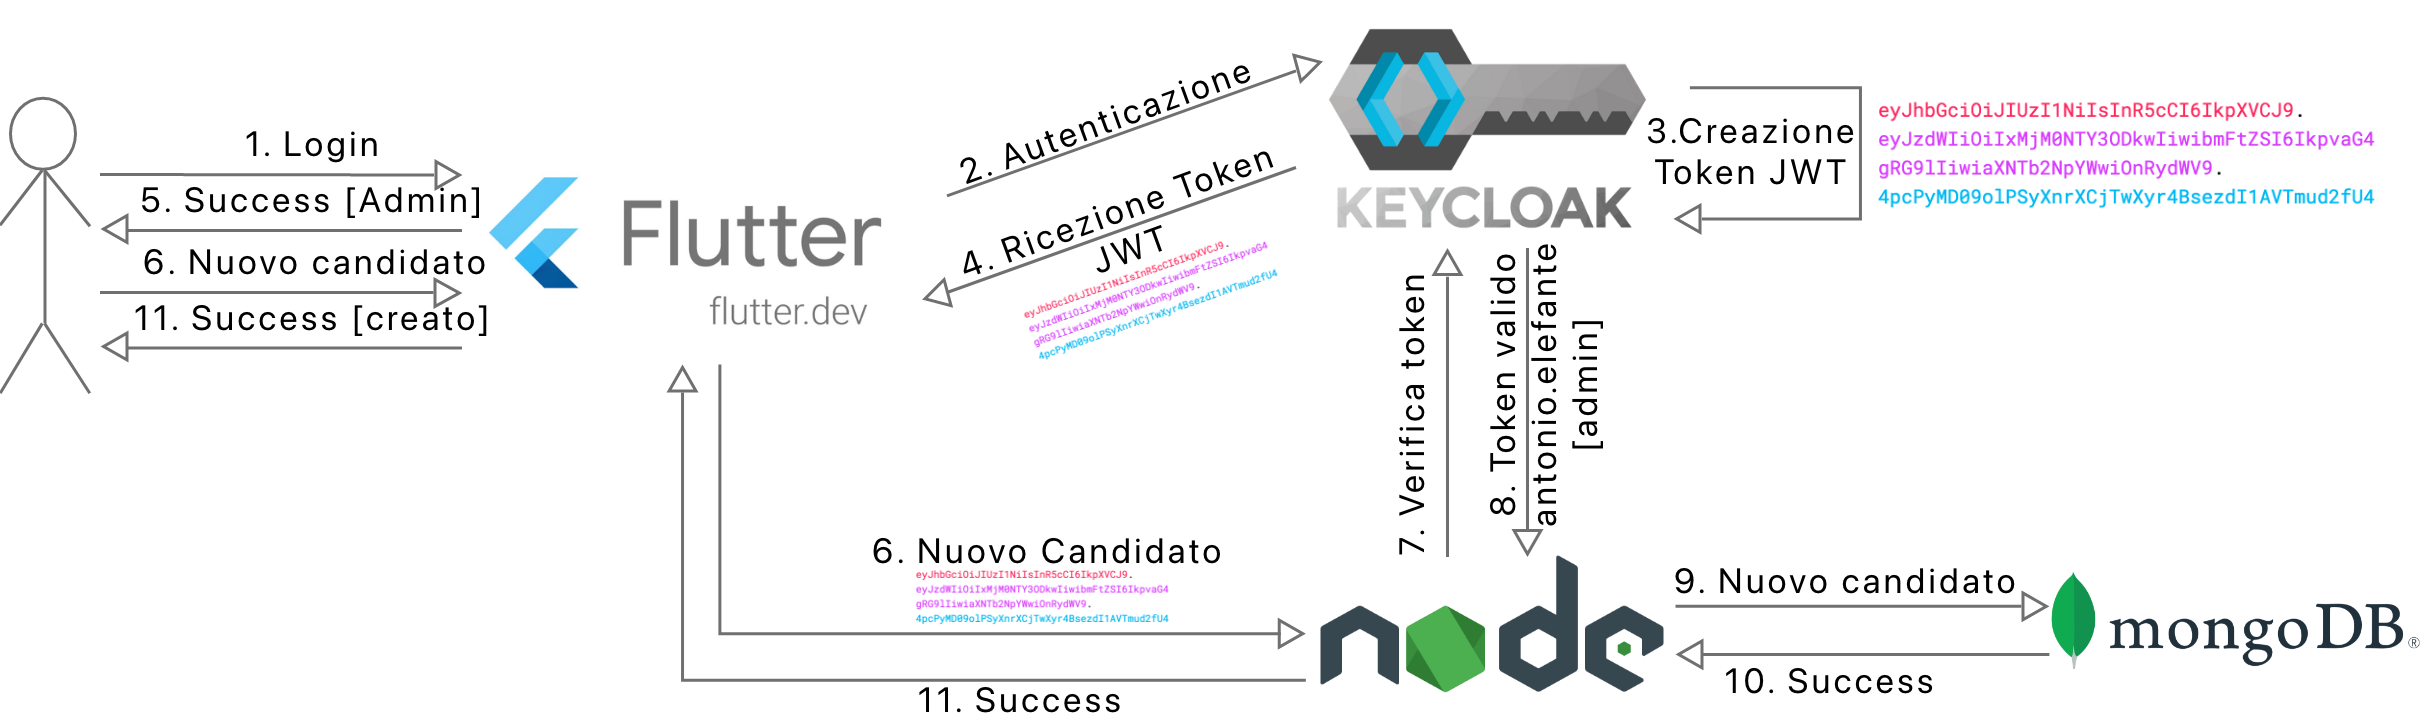
\includegraphics[width=1.5\linewidth]{flow.png}
};
\end{tikzpicture}

\newpage

Da qui in poi invece sono riportate le schermate che gli utenti Salvatore Ambrosio[USER] e l'utente Antonio Elefante[ADMIN] dovranno far utilizzo per interagire con il sistema.
\bigbreak
\begin{minipage}{\linewidth}
    \vspace{2mm}
    \centering
    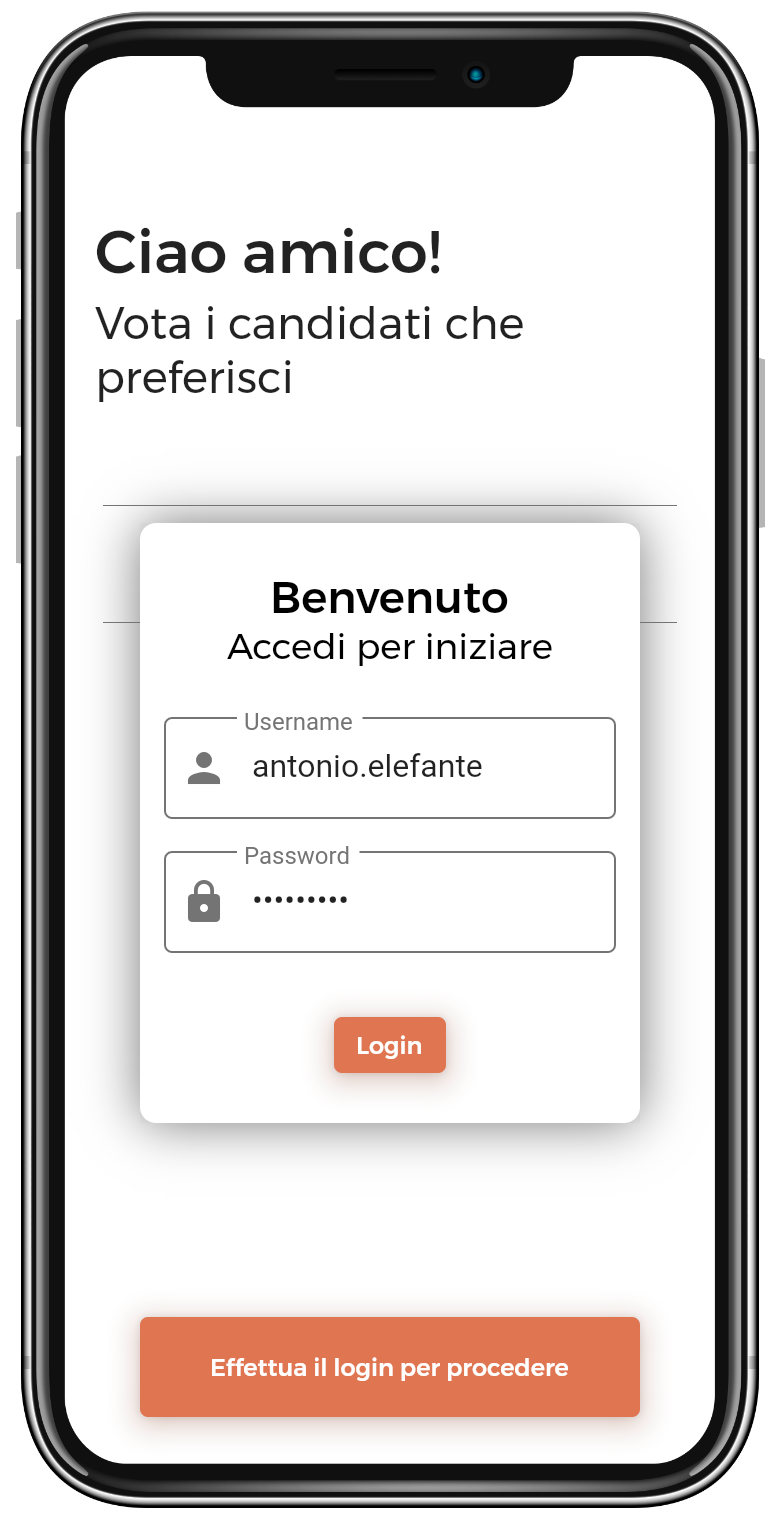
\includegraphics[width= 0.5 \linewidth]{2.png}
    \captionof{figure}{Accesso utente Admin}
    \vspace{2mm}
\end{minipage}

\begin{minipage}{\linewidth}
    \vspace{2mm}
    \centering
    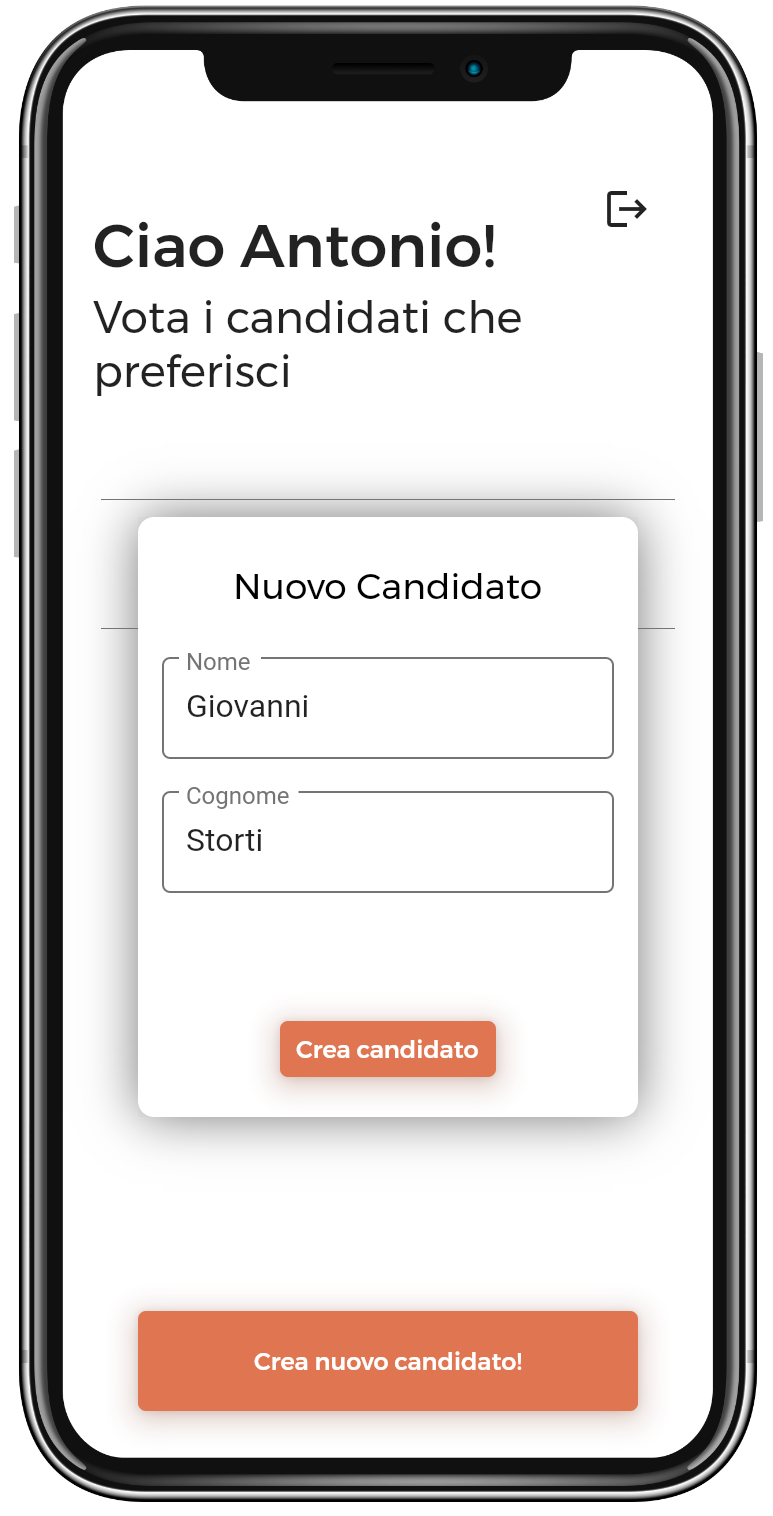
\includegraphics[width= 0.5 \linewidth]{3.png}
    \captionof{figure}{Creazione nuovo candidato}
    \vspace{2mm}
\end{minipage}

\begin{minipage}{\linewidth}
    \vspace{2mm}
    \centering
    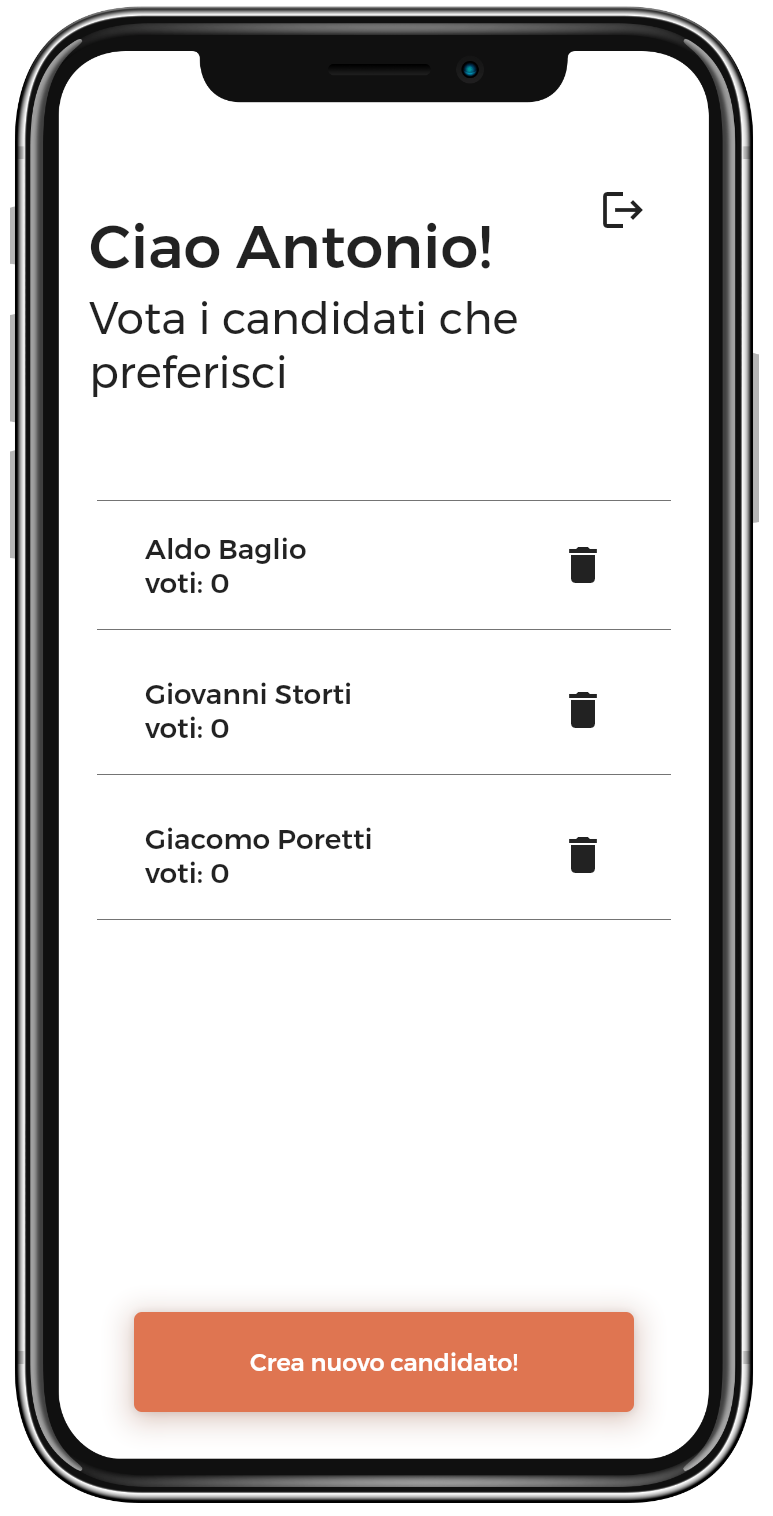
\includegraphics[width= 0.5 \linewidth]{4.png}
    \captionof{figure}{Lista candidati in visualizzazione Amministratore}
    \vspace{2mm}
\end{minipage}

\begin{minipage}{\linewidth}
    \vspace{2mm}
    \centering
    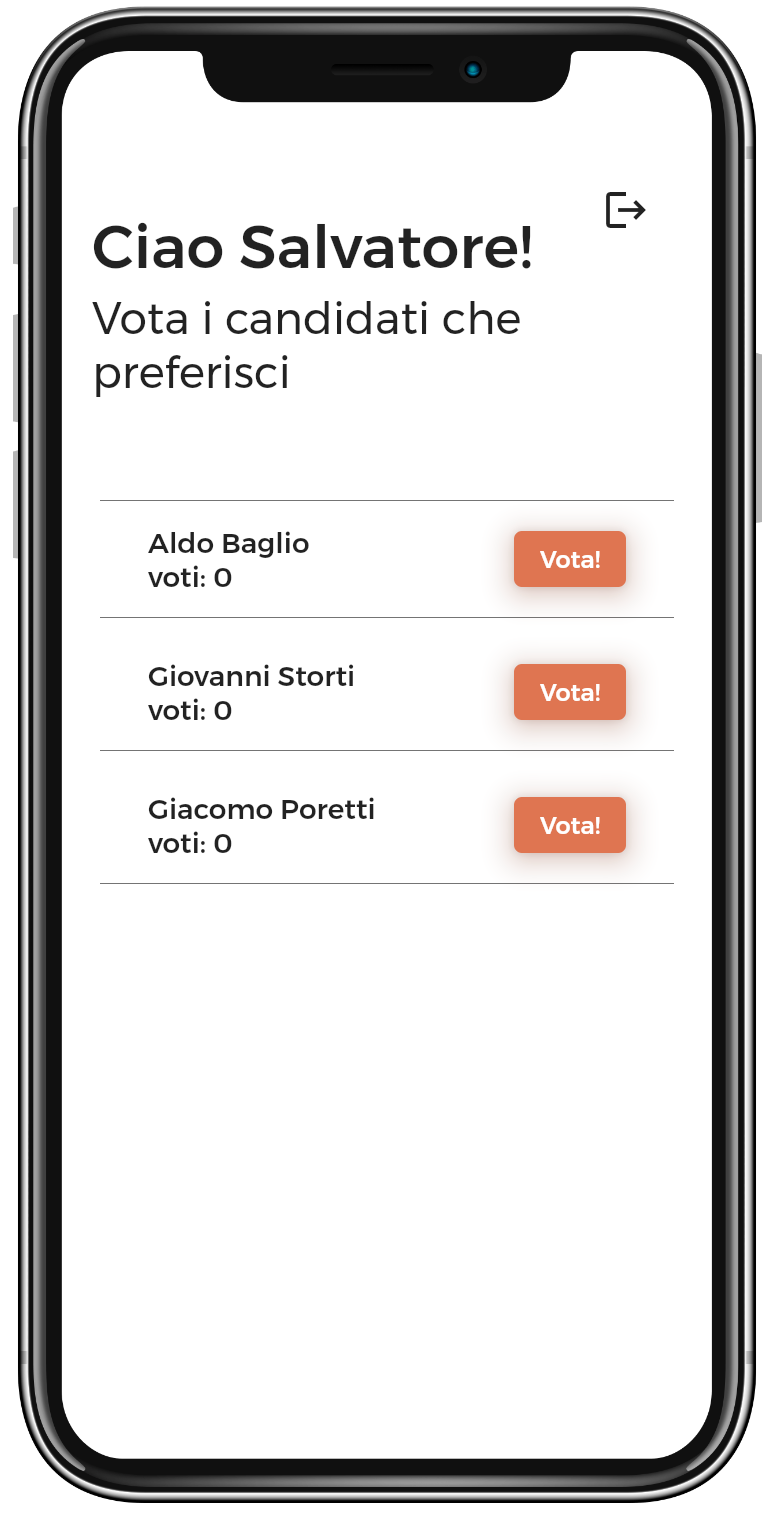
\includegraphics[width= 0.5\linewidth]{5.png}
    \captionof{figure}{Lista candidati in visualizzazione Utente}
    \vspace{2mm}
\end{minipage}

\begin{minipage}{\linewidth}
    \vspace{2mm}
    \centering
    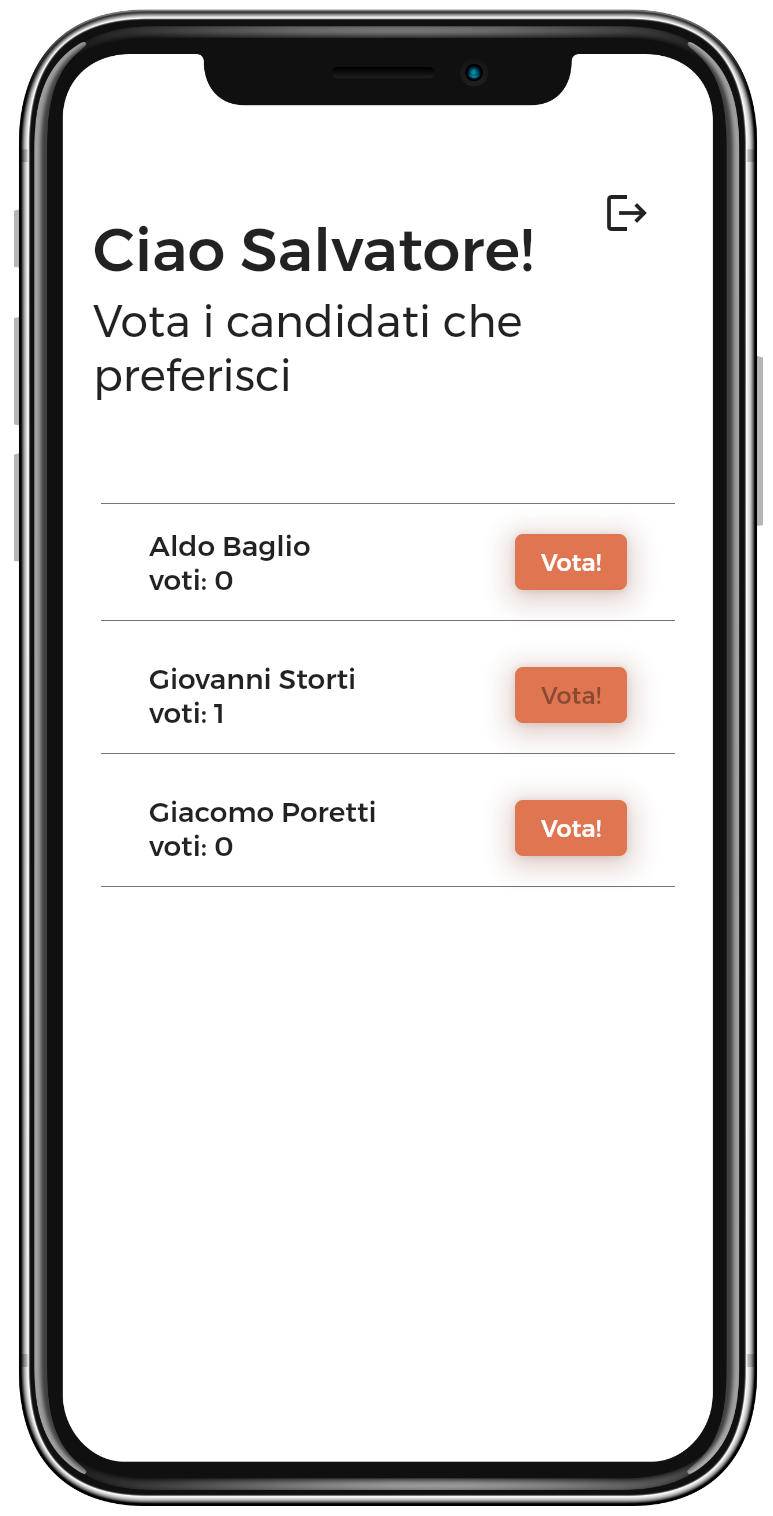
\includegraphics[width= 0.5 \linewidth]{6.png}
    \captionof{figure}{Votazione candidato Giovanni Storti}
    \vspace{2mm}
\end{minipage}

\begin{minipage}{\linewidth}
    \vspace{2mm}
    \centering
    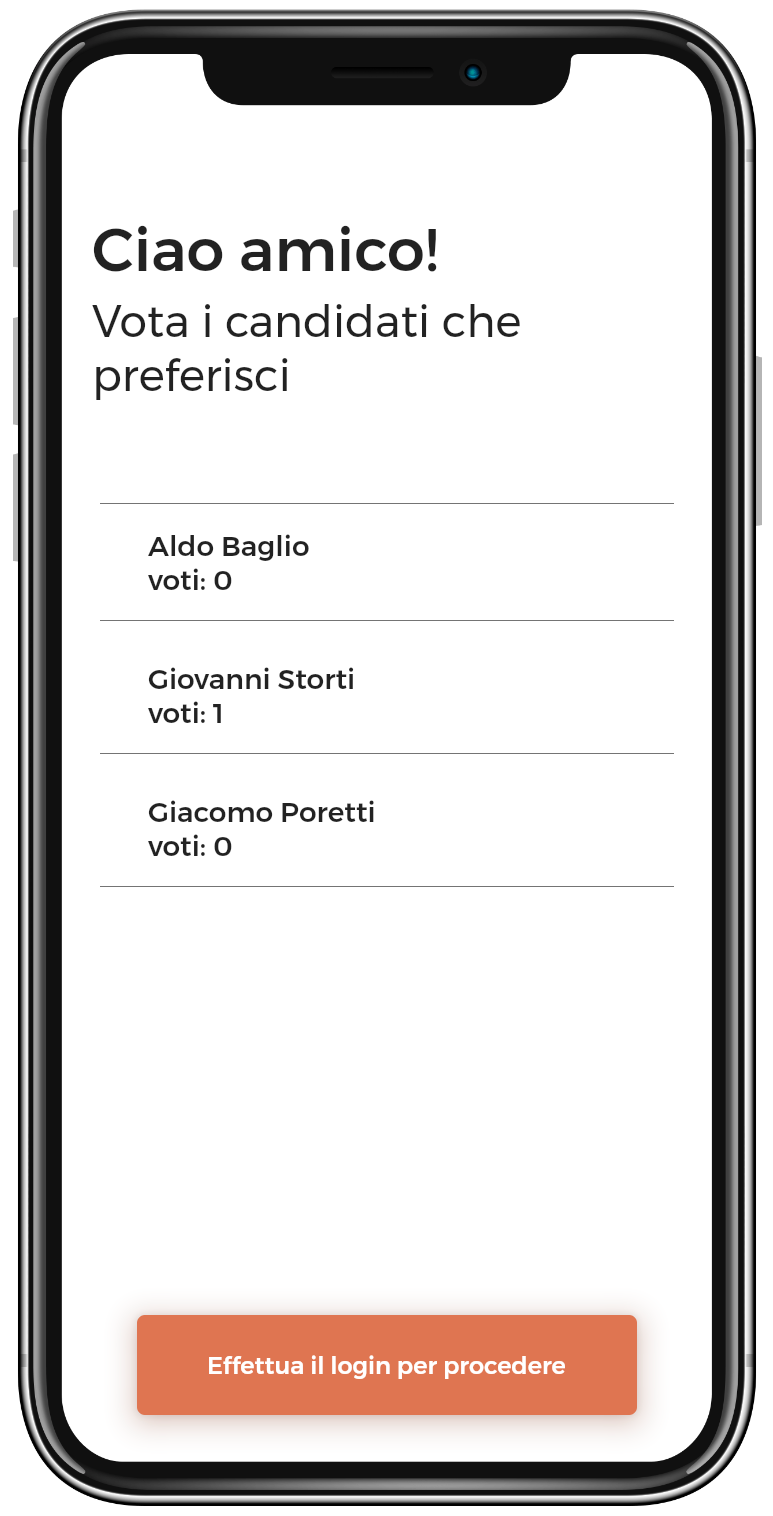
\includegraphics[width= 0.5\linewidth]{1.png}
    \captionof{figure}{Lista candidati in visualizzazione Anonima}
    \vspace{2mm}
\end{minipage}
\newpage
\subsection{Come testare il prodotto finale}

Una volta effettuato l'accesso ai files associati a tale documentazione, comunque disponibili in maniera pubblica al seguente link \href{https://github.com/antonioacademy10/progetto-soasec}{\underline{GitHub}}, è possibile tramite docker avviare i 3 differenti server:

\begin{itemize}
    \item Server NodeJS (API)
    \item Server Keycloak (Authentication + Authorization)
    \item Server MongoDB (Persistenza dei dati)
\end{itemize}

Per far ciò basterà recarsi tramite terminale nella cartella del progetto ed eseguire il comando:
\begin{listing}[h!]
\begin{minted}[frame=single,
               framesep=3mm,
               bgcolor=white,
               numbersep=-10pt,
               ]{bash}
docker-compose up
\end{minted} 
\end{listing}
\FloatBarrier

\bigbreak

Il quale si occuperà di scaricare (ed eseguire) tutti i container necessari per testare il progetto finale. Una volta fatto ciò basterà quindi recarsi al sito \href{https://antonioacademy10.github.io/progetto-soasec-github-pages/}{\underline{GitHub Pages}} (preferibilmente da Desktop/Tablet) per accedere all'interfaccia front-end e quindi interagire con il sistema ricordando che:
\begin{table}[h]
\centering
\begin{tabular}{|c|c|c|}
\hline
\textbf{Username} & \textbf{Password} & \textbf{Role} \\ \hline
antonio.elefante    & 123456789 & Amminstratore   \\ \hline
salvatore.ambrosio    & Password123! & User  \\ \hline
\end{tabular}
\captionof{table}{Credenziali utente con relativo ruolo}
\end{table}
\FloatBarrier

Inoltre è predisposta la possibilità di osservare in maniera anonima la lista dei candidati senza ovviamente però poter procedere con la votazione.

\bigbreak
\pagestyle{empty} 
\thispagestyle{empty} 
\listoffigures
\thispagestyle{empty} 
\listoftables
\thispagestyle{empty} 


\end{document}


















